

\chapter{Diseño e implementación} % Main chapter title

\label{Chapter3} % Change X to a consecutive number; for referencing this chapter elsewhere, use \ref{ChapterX}



En este capítulo se presentan los detalles del diseño de los nodos sensores y actuadores que conforman el trabajo, como así también los del software seleccionado.

\section{Arquitectura de la solución}
\label{sec:Arquitectura de la solución}

%Como se observa en la figura \ref{fig:blockdiagram}, el invernadero inteligente está compuesto por un conjunto de subsistemas encargados de las diferentes funciones de medición y control de variables, una aplicación central y un sistema que permita el acceso remoto de forma segura.

Para la implementación del prototipo propuesto en el trabajo se requirió la construcción de diferentes subsistemas encargados de las múltiples funciones dentro del invernadero inteligente. Cada uno de ellos opera en forma independiente del resto y todos se comunican con una aplicación central mediante una red inalámbrica. 
Para garantizar el acceso de los usuarios desde Internet se desarrolló una interfaz de acceso remoto.





\subsection{Componentes del sistema}
\label{Componentes del sistema}

En la figura \ref{fig:blockdiagram} se observa el diagrama en bloques de la arquitectura diseñada, que está compuesta por los siguientes elementos: 

\begin{itemize}
\item Sistema de monitoreo y control de clima, formado por dos módulos:
\begin{itemize}
\item Sensores de temperatura y humedad con sus correspondientes microcontroladores.
\item Unidad de control de temperatura y humedad comprendida por un microcontrolador, relé y ventiladores. 
\end{itemize}
Los sensores miden la temperatura y humedad ambiente en el invernadero y envían estos valores a la aplicación central por medio del microcontrolador. De acuerdo con los datos recibidos, la aplicación determina si es necesario emitir una señal para que la unidad de control encienda los ventiladores.



\item Sistema de control de riego, dividido en dos partes:
\begin{itemize}
\item Conjunto de sensores de humedad de suelo con sus respectivos microcontroladores.
\item Unidad de control de riego constituida por un microcontrolador, relés, bomba de agua y válvulas.
\end{itemize}

Los sensores envían las mediciones a la aplicación central que se encarga de procesarlas. En caso de ser necesario, se disparan las señales de encendido a través de la unidad de control. Primero se activa la válvula que corresponda y luego se enciende la bomba de agua para comenzar el riego. El orden de estas actividades es importante para evitar daños en la bomba o las cañerías.

\item Aplicación central: constituye el cerebro del invernadero y es la encargada de almacenar los parámetros de configuración de los diversos sensores y actuadores, procesar los mensajes recibidos, disparar acciones y alertas y visualizar el estado general.

\item Sistema de acceso remoto: permite a los usuarios obtener reportes del sistema en forma segura desde Internet.   
\end{itemize}



\begin{figure}[h]
	\centering
	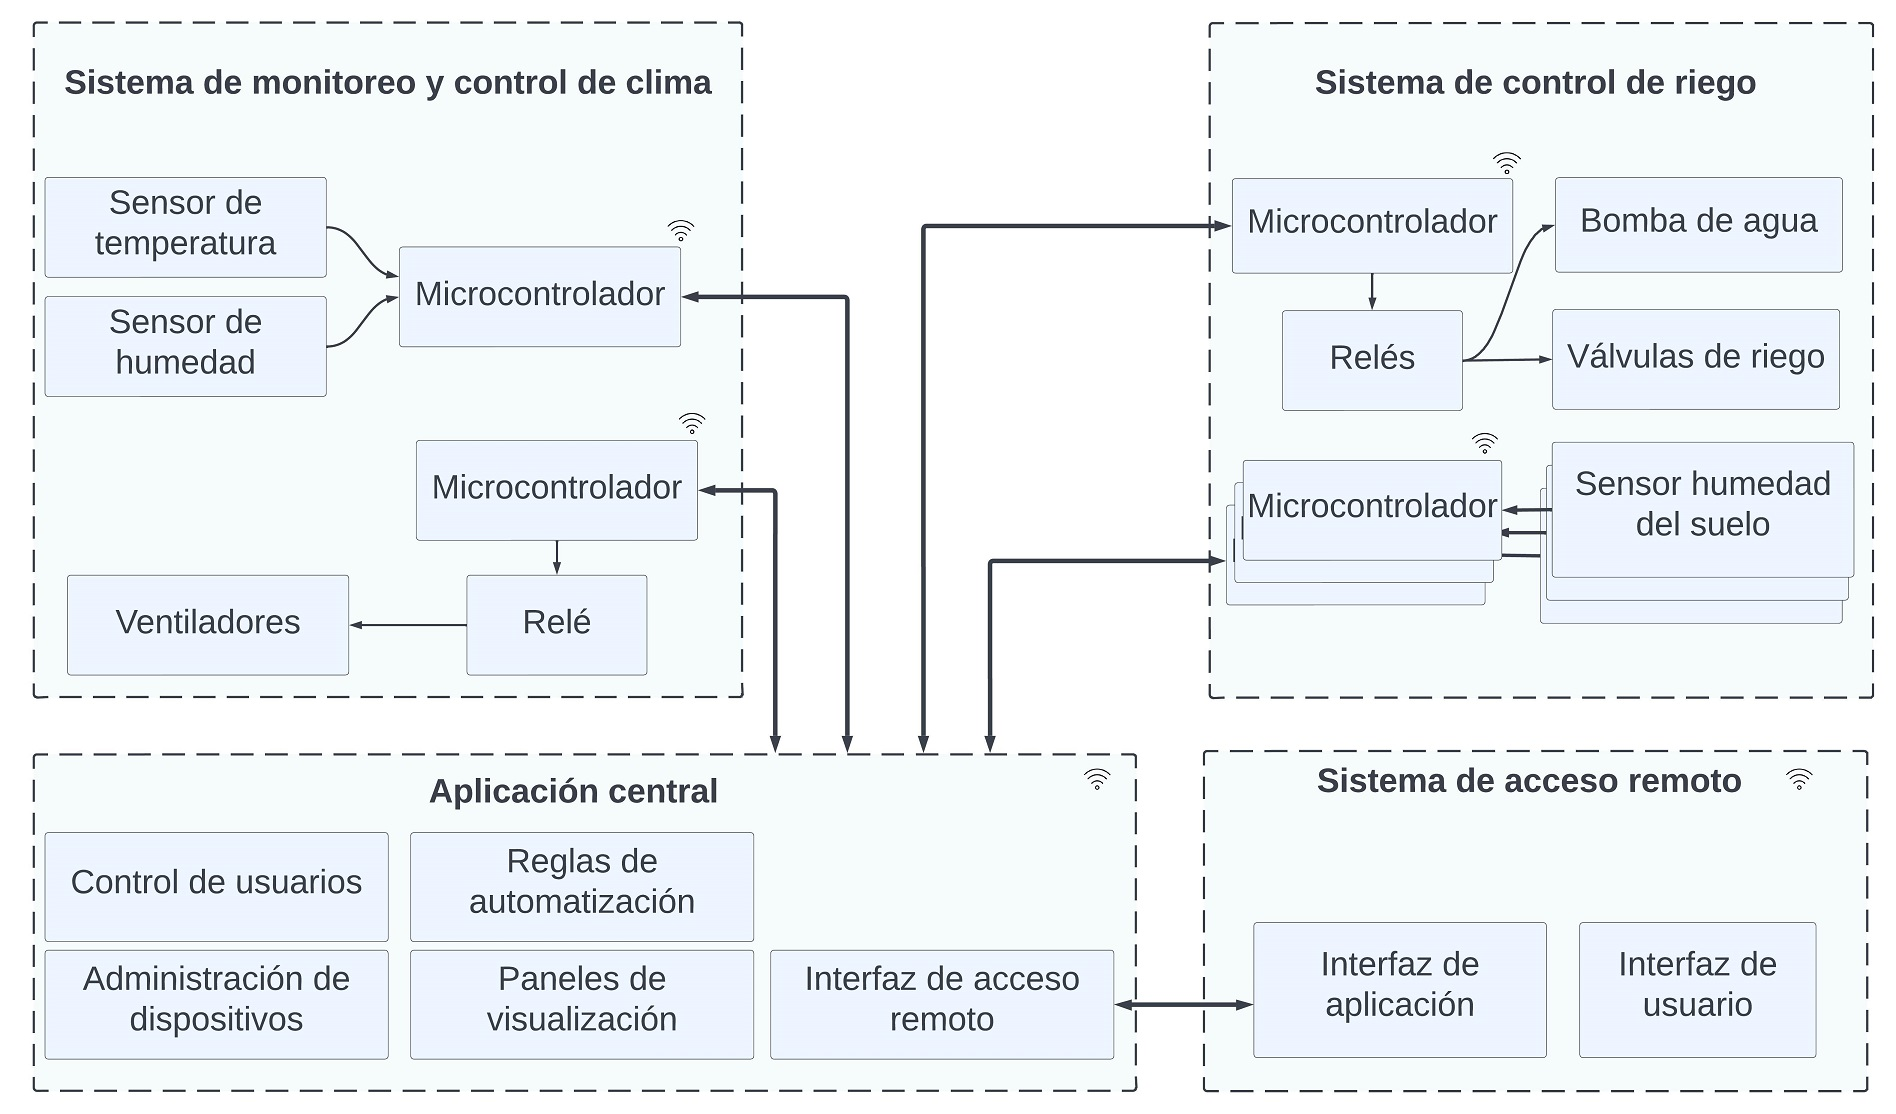
\includegraphics[width=1.0\textwidth]{./Figures/blockdiagram4.jpg}
	\caption[Arquitectura del sistema.]{Arquitectura del sistema.}
	\label{fig:blockdiagram}

\end{figure}


\subsection{Protocolos de comunicación}
\label{Protocolos de comunicación}
%\textit{Aquí se describe cómo se comunican los sistemas con la aplicación central y los protocolos usados en cada caso.}

%En la selección del software de la aplicación central se contempló la compatibilidad con múltiples protocolos de comunicación. Sin embargo limitaciones de configuración específicas, tal como el tiempo de retención de los mensajes en las colas de MQTT, forzaron el utilizar diferentes protocolos dependiendo del módulo en cuestión. Otro factor condicionante, como se detalla en la sección \ref{sec:Ciberseguridad del sistema}, fue el carecer de una CA que emita certificados que todos los componentes puedan confiar.

En esta sección se describe cómo se comunican los sistemas con la aplicación central y los protocolos usados en cada caso. En la figura \ref{fig:blockprotos} se aprecia un esquema simplificado que ilustra dichas interacciones.

Si bien los módulos de hardware y el software soportan una gran variedad de protocolos,  se implementó MQTT en la mayoría de los casos conforme a los requerimientos. En algunas situaciones donde esto no fue técnicamente posible, se utilizó HTTP. Adicionalmente, para garantizar la seguridad de las comunicaciones, se incorporó un certificado autofirmado TLS en el servidor.

\begin{figure}[h]
	\centering
	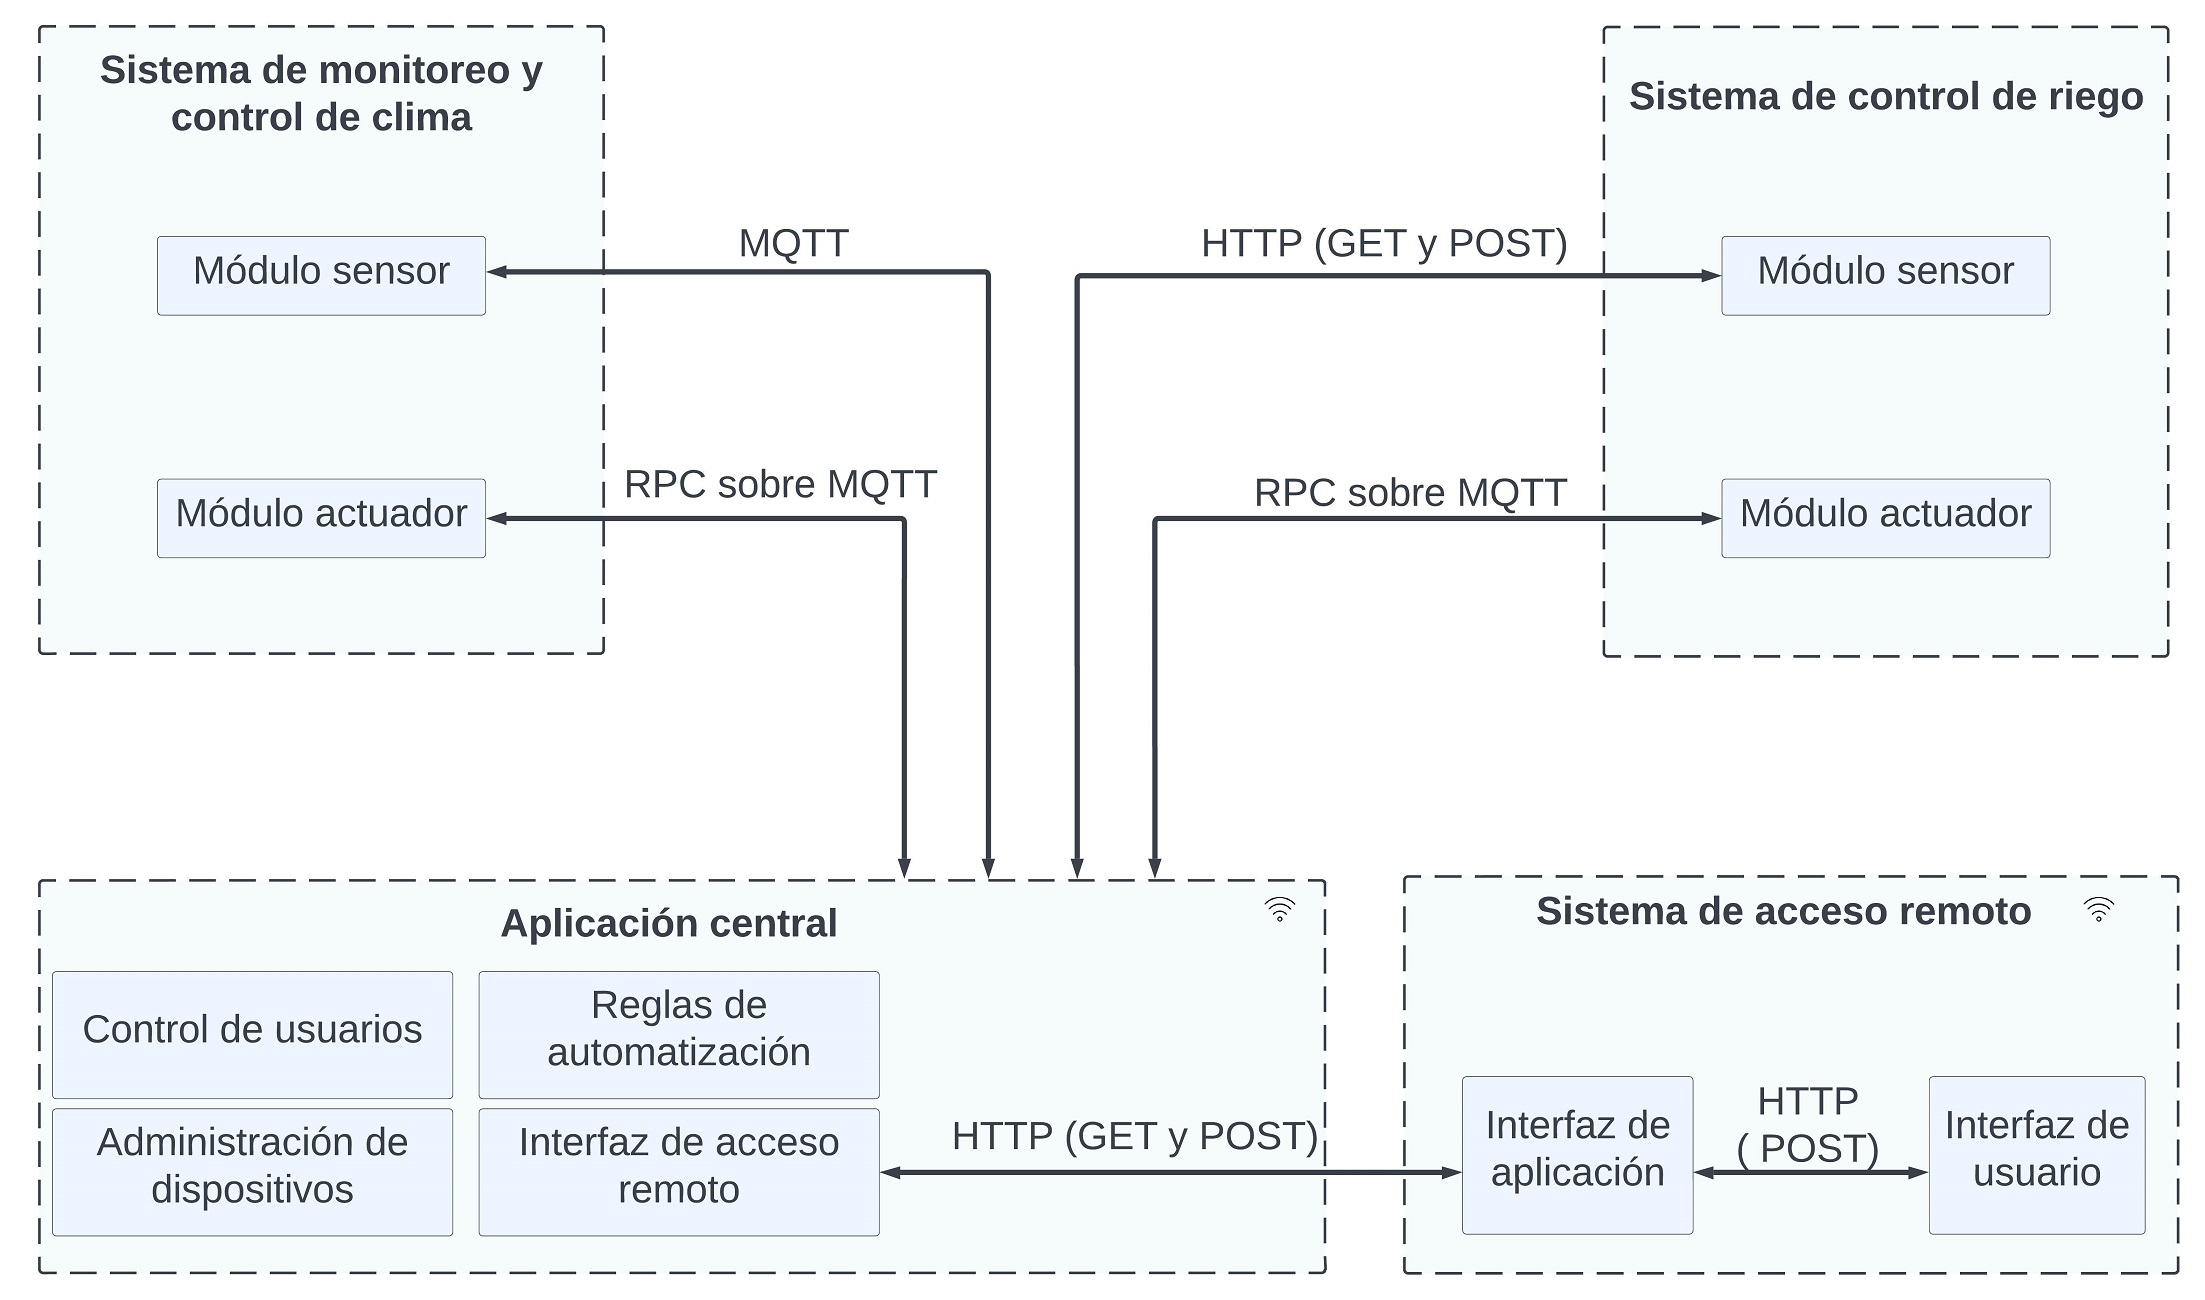
\includegraphics[width=1.0\textwidth]{./Figures/blockproto.jpeg}
	\caption[Protocolos de comunicación entre módulos.]{Protocolos de comunicación entre módulos.}
	\label{fig:blockprotos}
\end{figure}


\pagebreak
Las interacciones principales entre los bloques componentes son:
 
 \begin{itemize}
	\item Sistema de monitoreo y control de clima: las comunicaciones se realizan exclusivamente con la aplicación central.
	El módulo sensor envía las mediciones realizadas por medio de MQTT y en caso de requerir una acción, la aplicación central comanda el encendido de los ventiladores por medio de un mensaje enviado por RPC \citep{rfc1057} sobre MQTT.
	
	\item Sistema de control de riego: las comunicaciones se realizan con la aplicación central de manera bidireccional.
	El módulo sensor efectúa dos conexiones, una para el envío de las mediciones y otra para recibir valores de atributos tales como la duración del tiempo de riego. Debido a limitaciones en la configuración de la persistencia de los mensajes en las colas de MQTT, se optó por utilizar llamadas HTTP (GET y POST) para realizarlas.
	Al igual que en el control de clima, la aplicación central inicia el riego por medio de mensajes RCP sobre MQTT hacia el controlador de la bomba y de las válvulas.
	
	\item Sistema de acceso remoto: la interfaz se comunica con la aplicación por medio de pedidos HTTP GET y POST para consultar el reporte de estado de los diferentes componentes. A continuación este se envía hacia la interfaz de usuario por medio de una solicitud HTTP POST.
 
 
 
 
 \end{itemize}






\section{Detalle de los módulos de hardware}
\label{sec:Módulos de hardware}
En esta sección se describen en detalle los esquemas de conexión de los distintos módulos y las consideraciones de diseño y construcción empleadas. 

\subsection{Módulos sensores de humedad del suelo}
\label{Módulos sensores de humedad del suelo}


En el proyecto se desarrollaron dos configuraciones diferentes de módulos para medir la humedad del suelo en macetas de diverso tipo y tamaño. Ambas opciones utilizan el microcontrolador ESP8266, pero incorporan distintas cantidades de sensores. En la figura \ref{fig:soilschem1} se muestra el esquema de conexión para la versión simple (con un único sensor) y en la figura \ref{fig:soilschem2} se ilustra la configuración doble.

Si bien en el prototipo los sensores se conectaron a una fuente de alimentación, la configuración y conexión del sistema está optimizada para el uso de baterías. Esto se debe a que las sondas pueden estar desplegadas en múltiples ubicaciones dentro del invernadero y no siempre es posible conectarlas a la red eléctrica. 

El ahorro de energía necesario para permitir el uso de  baterías se logra a través de ciclos de apagado en los períodos donde no se realizan lecturas. A este mecanismo se lo que conoce como \textit{deep sleep} y una vez que el microcontrolador se encuentra en este estado, se requiere un pulso eléctrico en el pin de \textit{reset} para que retorne al modo activo. 
Para habilitar la reactivación se interconectan los pines D0 (GPIO16) y RST del chip ESP8266. Se logra así una reducción del consumo de energía a valores muy pequeños que rondan los 0,3 mA durante el período de inactividad.




\begin{figure}[!h]
     \centering
     \begin{subfigure}[b]{0.45\textwidth}
		\centering
		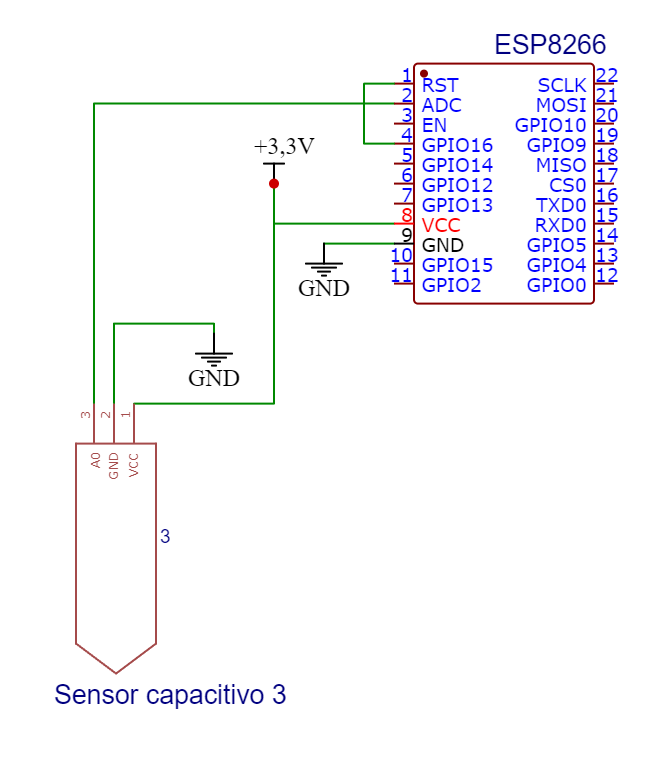
\includegraphics[width=0.9\textwidth]{./Figures/soil_schem_simple.png}
		\caption[Módulo sensor simple]{Módulo sensor simple.}
		\label{fig:soilschem1}
     \end{subfigure}
     \hfill
     \begin{subfigure}[b]{0.45\textwidth}
	\centering
		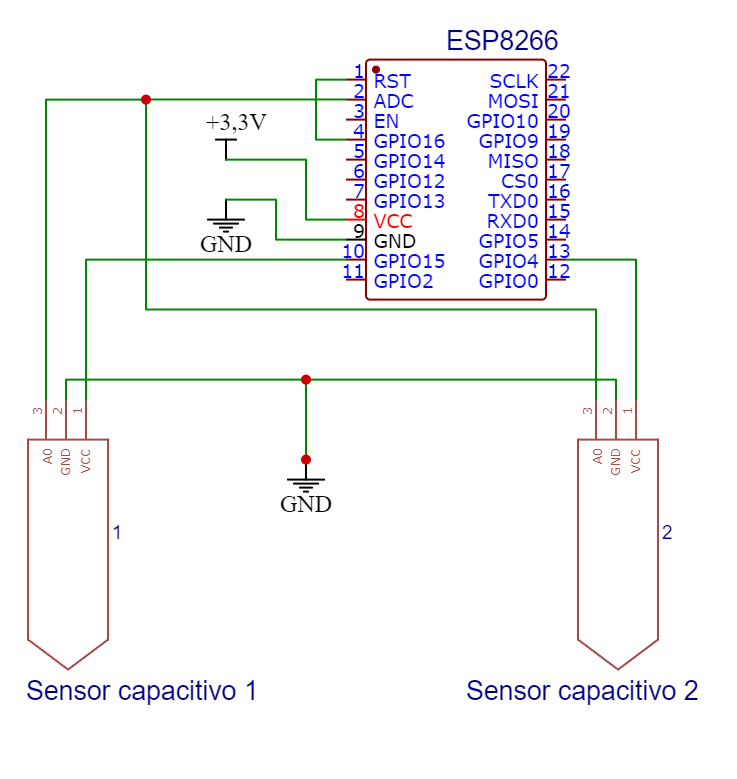
\includegraphics[width=1\textwidth]{./Figures/soil_schem_doble.png}
		\caption[Módulo sensor doble]{Módulo sensor doble.}
		\label{fig:soilschem2}
     \end{subfigure}
     \hfill
        \caption[Esquema de conexión de módulos sensores de humedad del suelo]{Esquema de conexión de módulos sensores de humedad del suelo.}	\label{fig:soilschem}
\end{figure}
%\begin{figure}[!h]
%	\centering
%	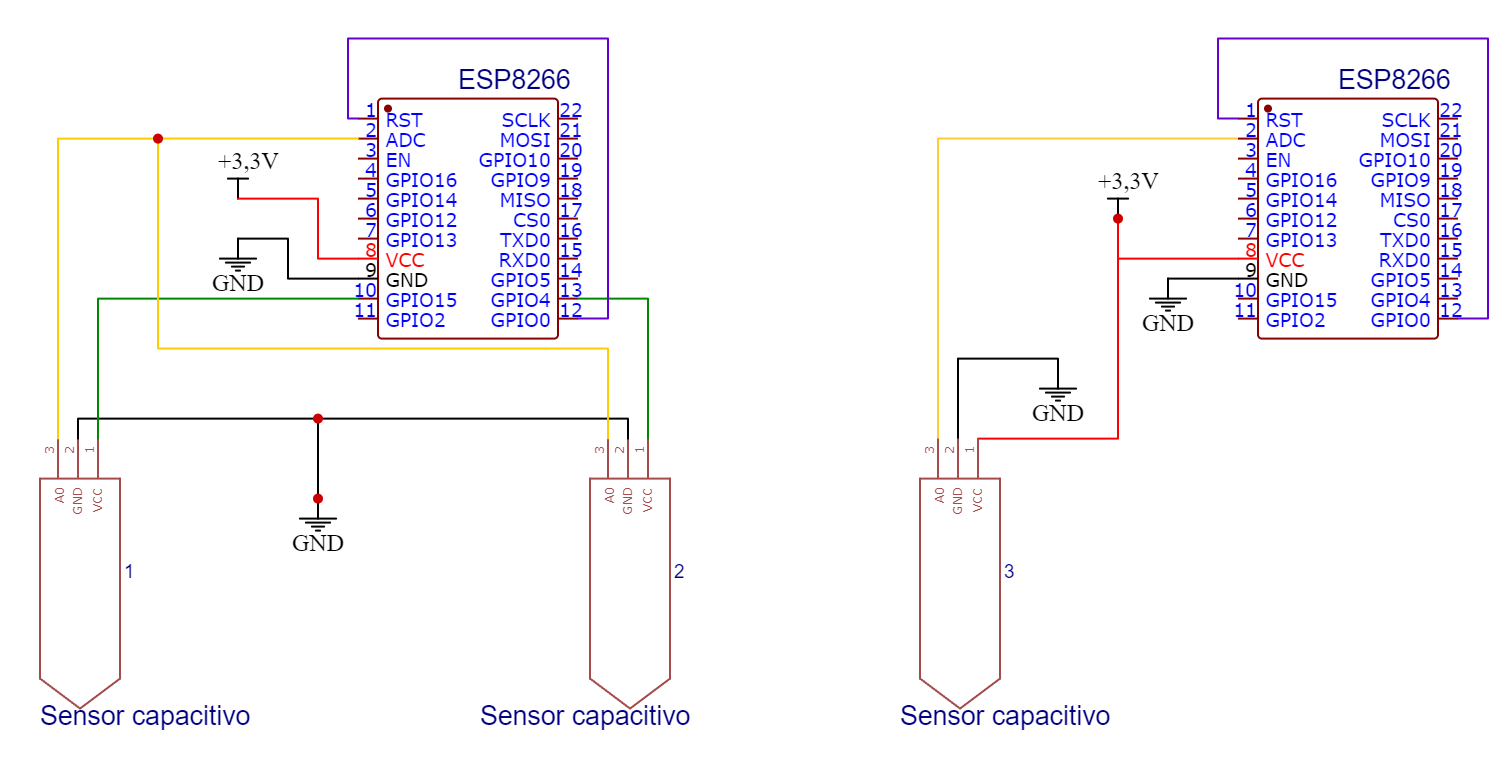
\includegraphics[width=1\textwidth]{./Figures/soil_schematic2.png}
%	\caption[Conexión del sensor de humedad del suelo]{Conexión del sensor de humedad del suelo.}
%	\label{fig:soilschem}
%\end{figure}

La integración de los componentes de los sensores se  realizó en forma manual por medio de placas de circuitos impresos (PCB) experimentales. En las figuras \ref{fig:soil1} y \ref{fig:soil2} se muestran los componentes empleados y un módulo ensamblado.

Dado que los sensores están expuestos a salpicaduras, se los recubrió con tubos adhesivos termocontraíbles que, al aplicarles calor, generan una protección a prueba de agua. Para el resguardo del chip ESP8266 se utilizó una caja de polipropileno transparente sellada. En las figuras \ref{fig:soil3} y \ref{fig:soil4} se muestran los componentes y sus protecciones. 

\begin{figure}[!h]
     \centering
     \begin{subfigure}[b]{0.45\textwidth}
		\centering
		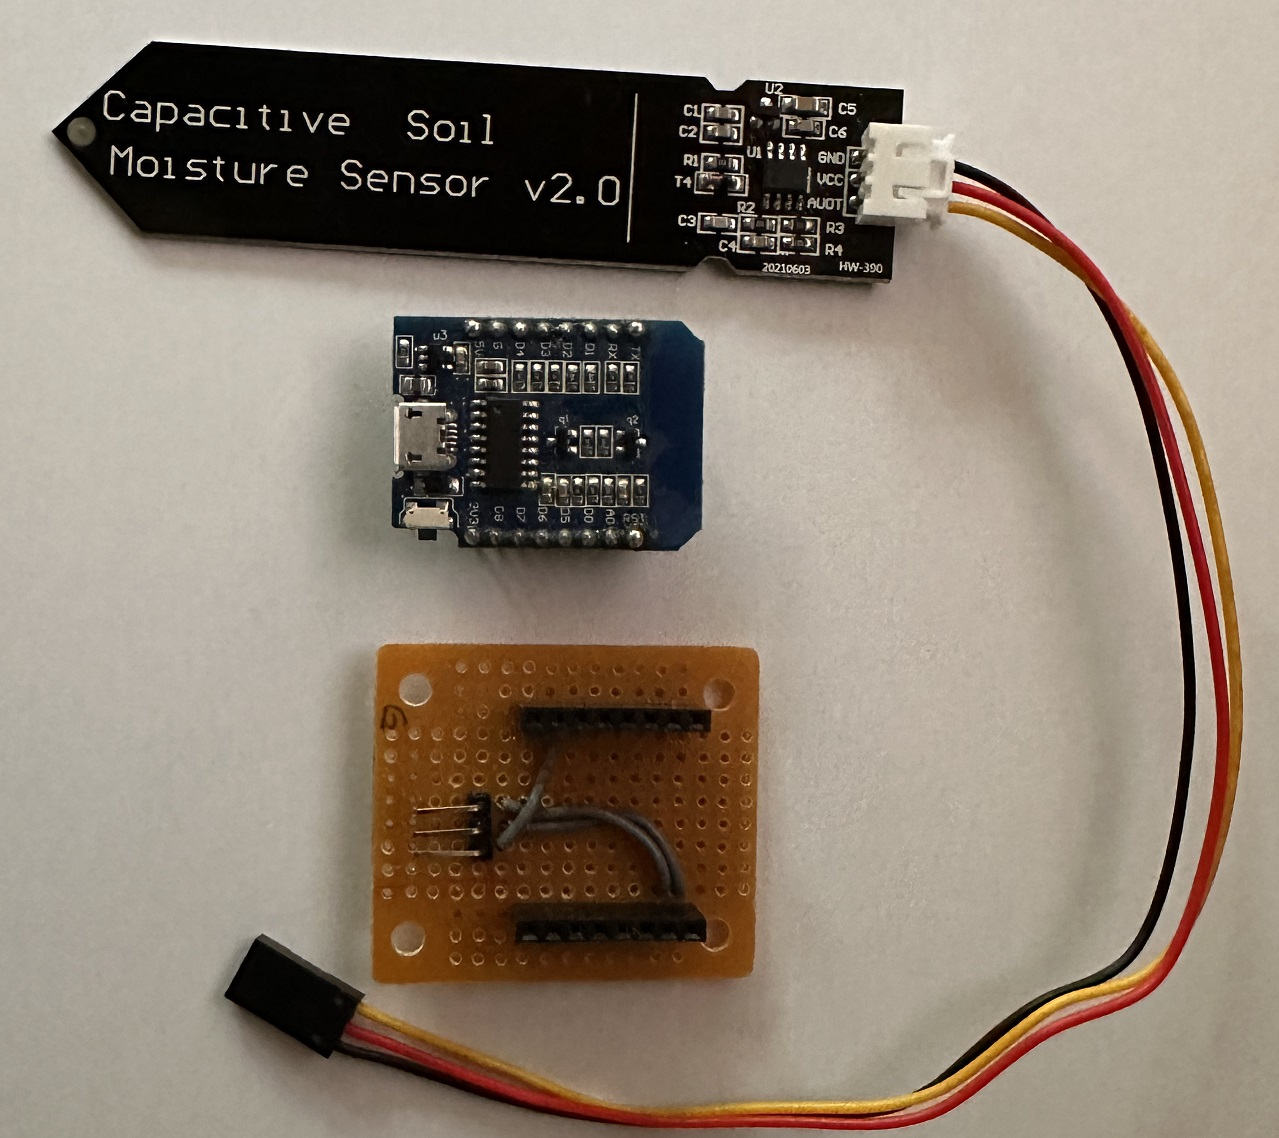
\includegraphics[width=0.80\textwidth]{./Figures/soil1.jpeg}
		\caption[Módulo con un sensor de humedad del suelo]{Módulo con un sensor de humedad del suelo.}
		\label{fig:soil1}
     \end{subfigure}
     \hfill
     \begin{subfigure}[b]{0.45\textwidth}
	\centering
		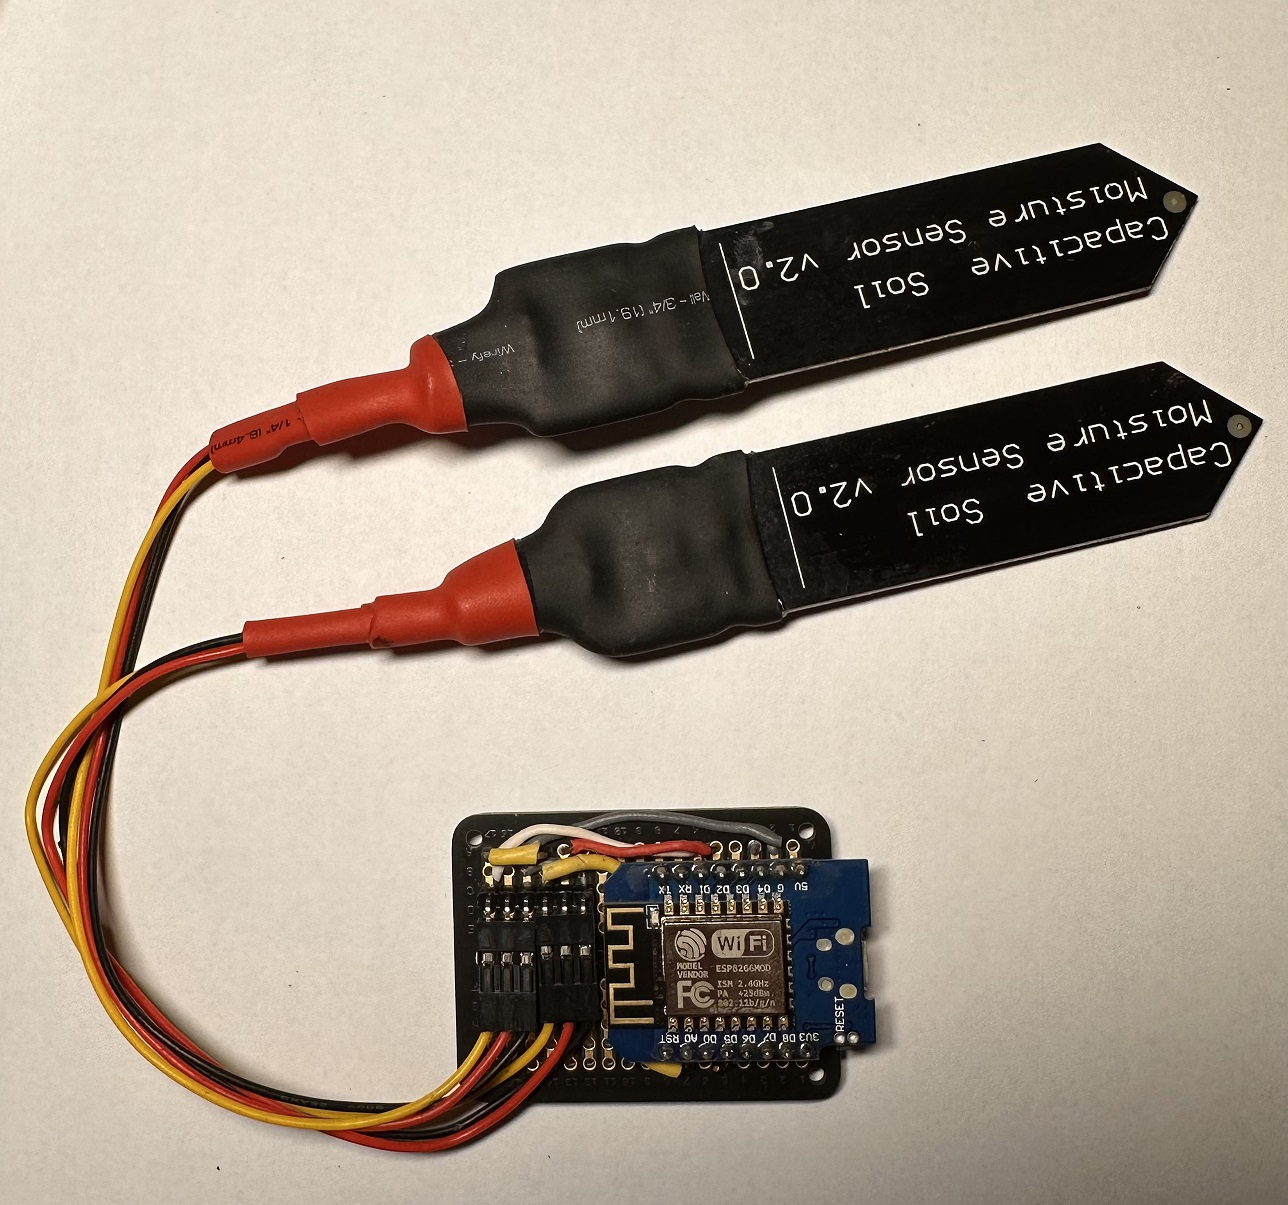
\includegraphics[width=0.80\textwidth]{./Figures/soil2.jpeg}
		\caption[Módulo con dos sensores de humedad del suelo]{Módulo con dos sensores de humedad del suelo.}
		\label{fig:soil2}
     \end{subfigure}
      \begin{subfigure}[b]{0.45\textwidth}
	\centering
		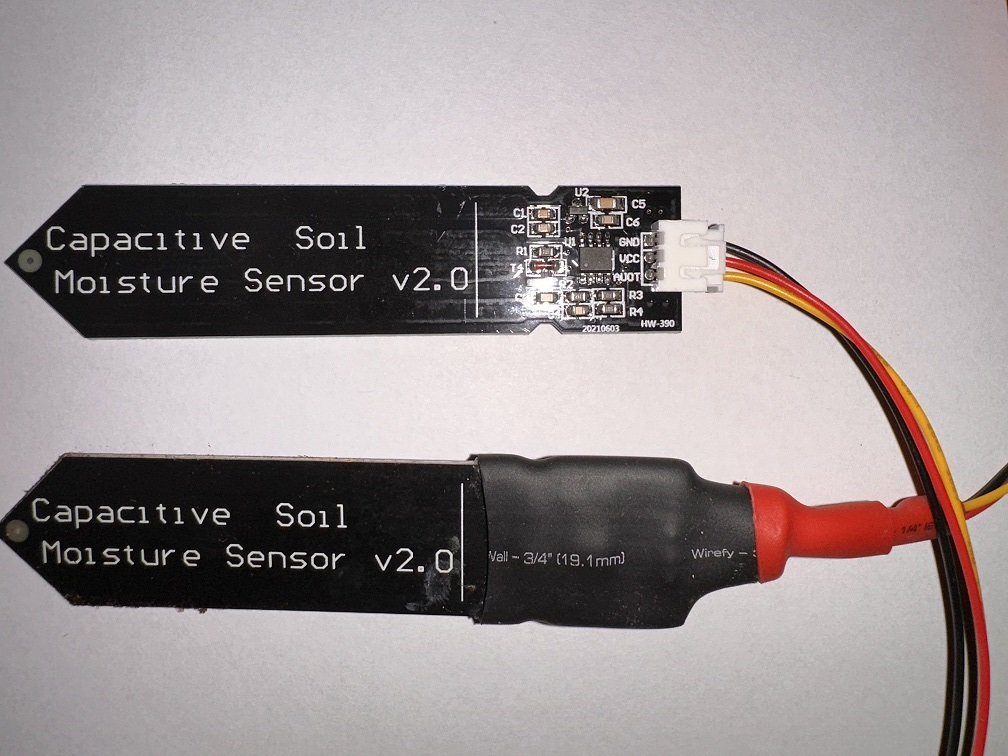
\includegraphics[width=0.80\textwidth]{./Figures/soil_compare.jpg}
		\caption[Detalle de protección de circuitos en los sensores]{Detalle de protección de circuitos en los sensores.}
		\label{fig:soil3}
     \end{subfigure}	
			\begin{subfigure}[b]{0.45\textwidth}
	\centering
		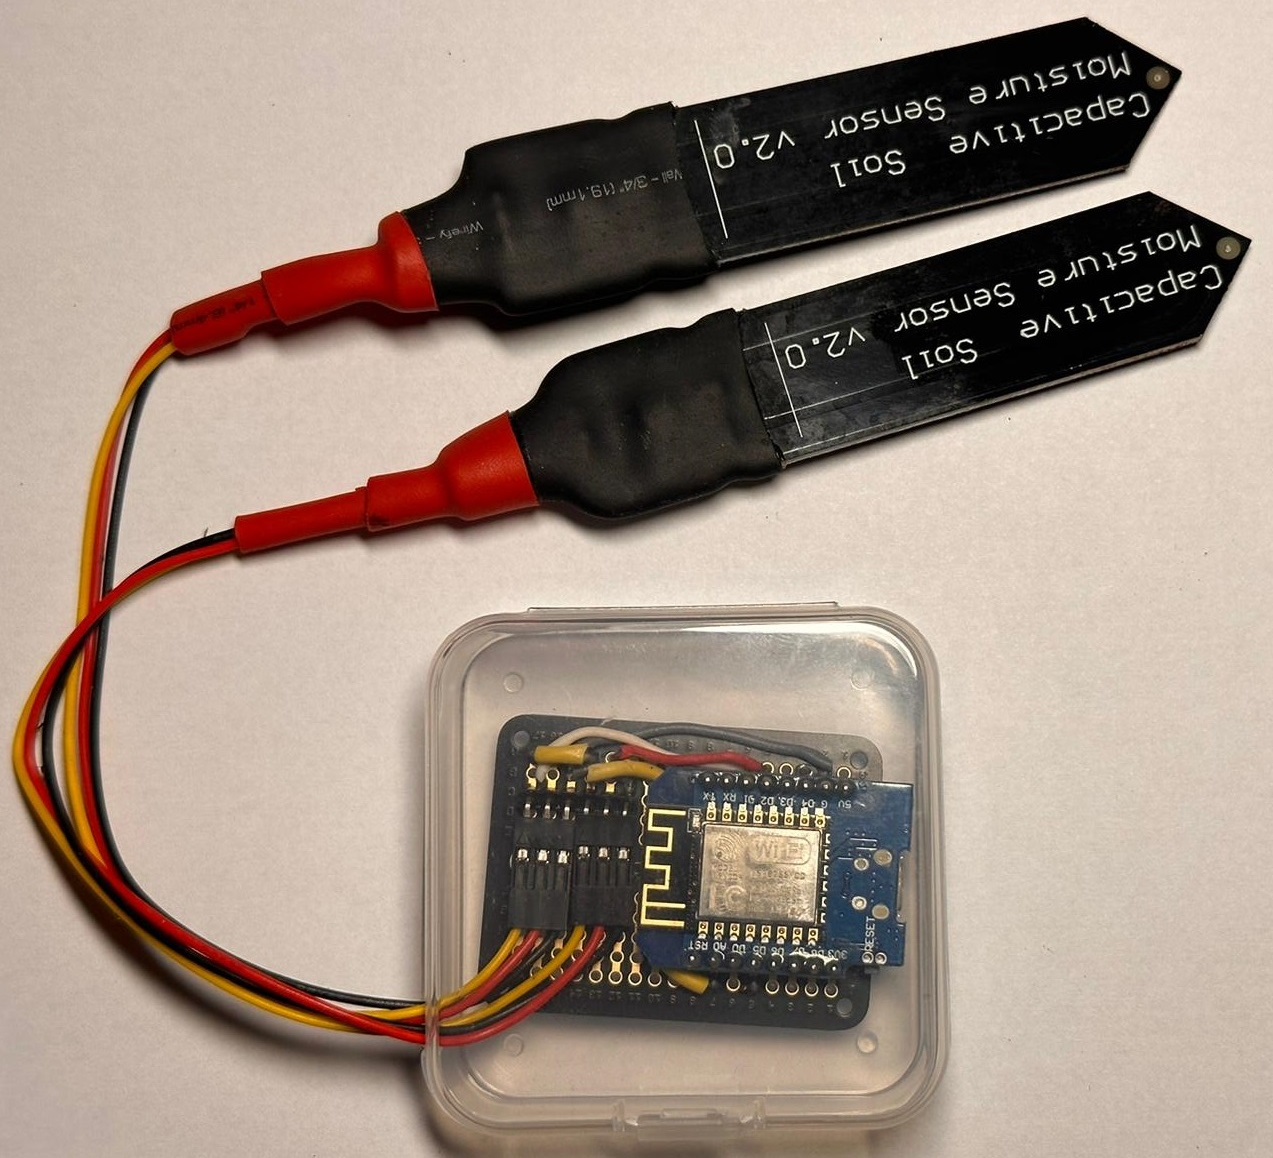
\includegraphics[width=0.80\textwidth]{./Figures/soil3.jpg}
		\caption[Módulo en su caja protectora]{Módulo en su caja protectora.}
		\label{fig:soil4}
     \end{subfigure}
     \hfill
        \caption[Módulos de sensores de humedad del suelo  empleados en el proyecto]{Módulo de sensores de humedad del suelo  empleados en el proyecto.}
        \label{fig:soilsenors}
\end{figure}


\pagebreak

\subsection{Módulo controlador del riego}
\label{Módulo controlador del riego}

Se compone de un microcontrolador ESP32, una placa de interfaz de relé de cuatro canales, una pantalla LCD/OLED SSH1106 y un regulador de voltaje DC-DC \textit{step down} LM2596. El esquema de conexiones entre estos componentes se detalla en la figura \ref{fig:riegochem}.

El módulo se alimenta con una fuente de 12 VDC y para energizar a los circuitos electrónicos el regulador LM2596 reduce la tensión a 5 VDC.

Para la construcción del prototipo se realizó la integración del microcontrolador con la pantalla LCD mediante una placa PCB experimental. Tanto para el módulo regulador de tensión como para el conjunto de relés, se emplearon circuitos preensamblados. En la figura \ref{fig:riego_control} se muestran los componentes, su conexionado y la versión final de la unidad dentro de una caja protectora.   


\begin{figure}[!h]
	\centering
	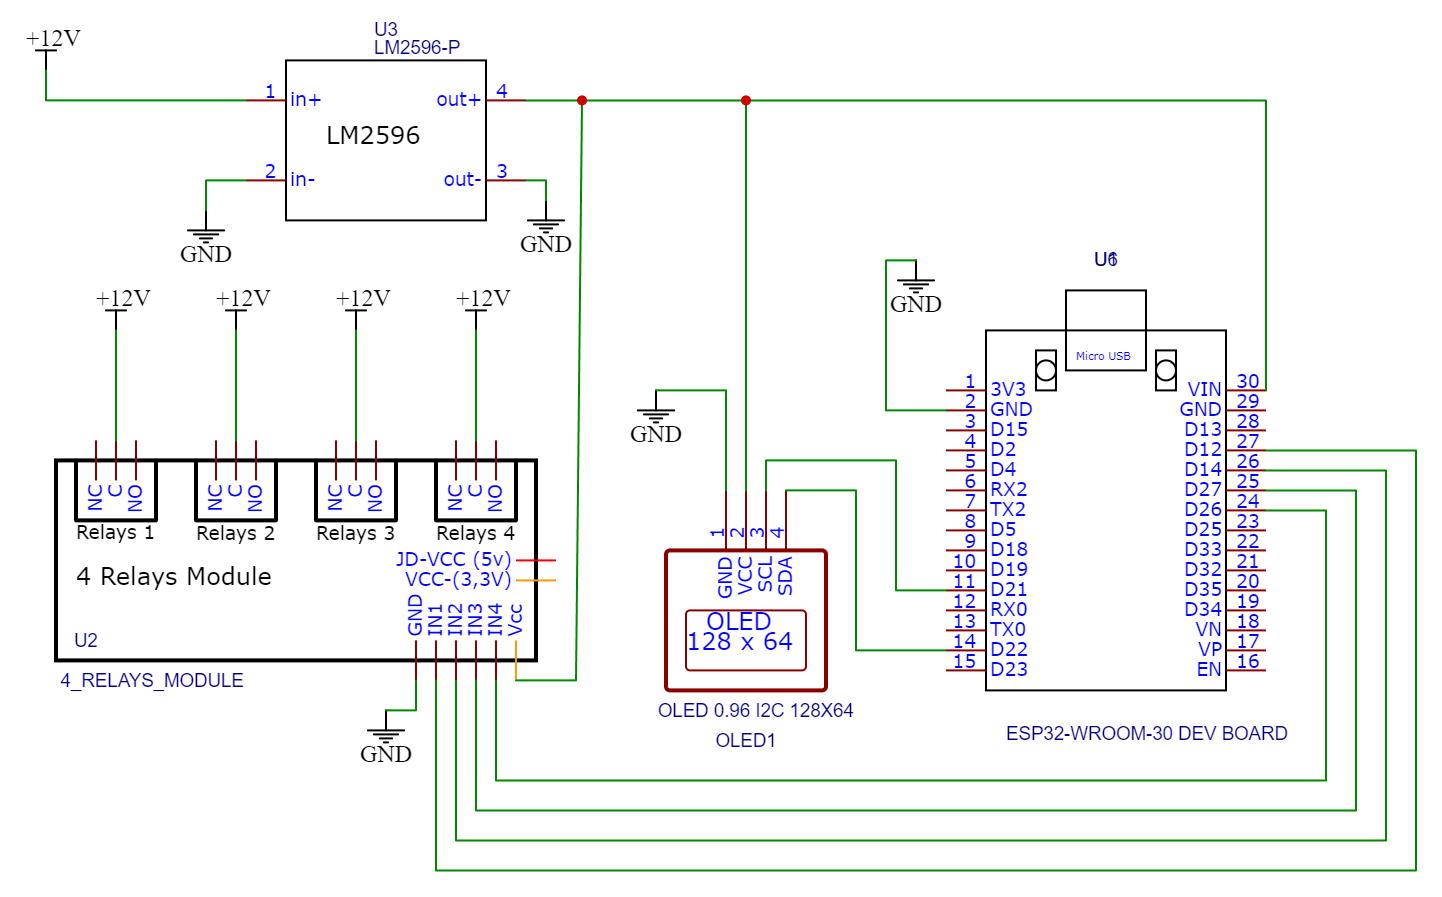
\includegraphics[width=0.9\textwidth]{./Figures/pump_schem.png}
	\caption[Conexión del módulo de control de riego]{Conexión del módulo de control de riego.}
	\label{fig:riegochem}
\end{figure}



\begin{figure}[!h]
     \centering
     \begin{subfigure}[b]{0.45\textwidth}
		\centering
		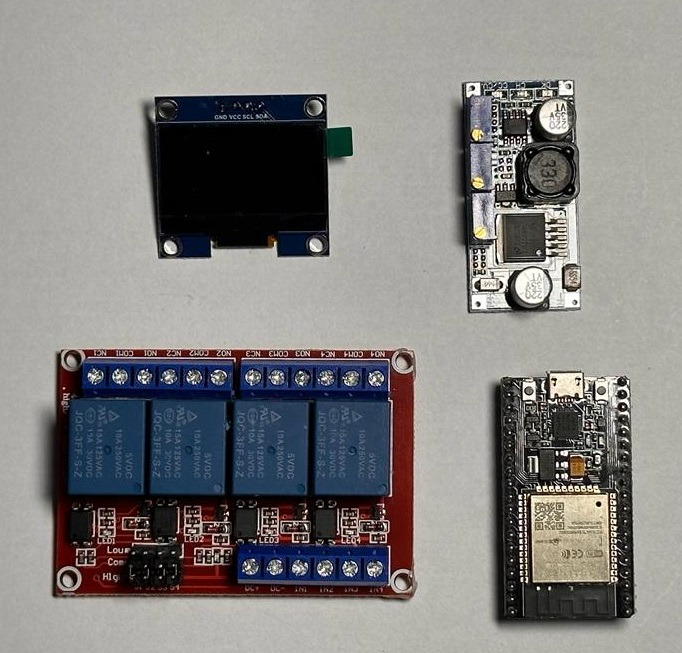
\includegraphics[width=0.8\textwidth]{./Figures/control_riego1.jpg}
		\caption[Detalle de los componentes]{Detalle de los componentes.}
		\label{fig:riego1}
     \end{subfigure}
     \hfill
     \begin{subfigure}[b]{0.45\textwidth}
	\centering
		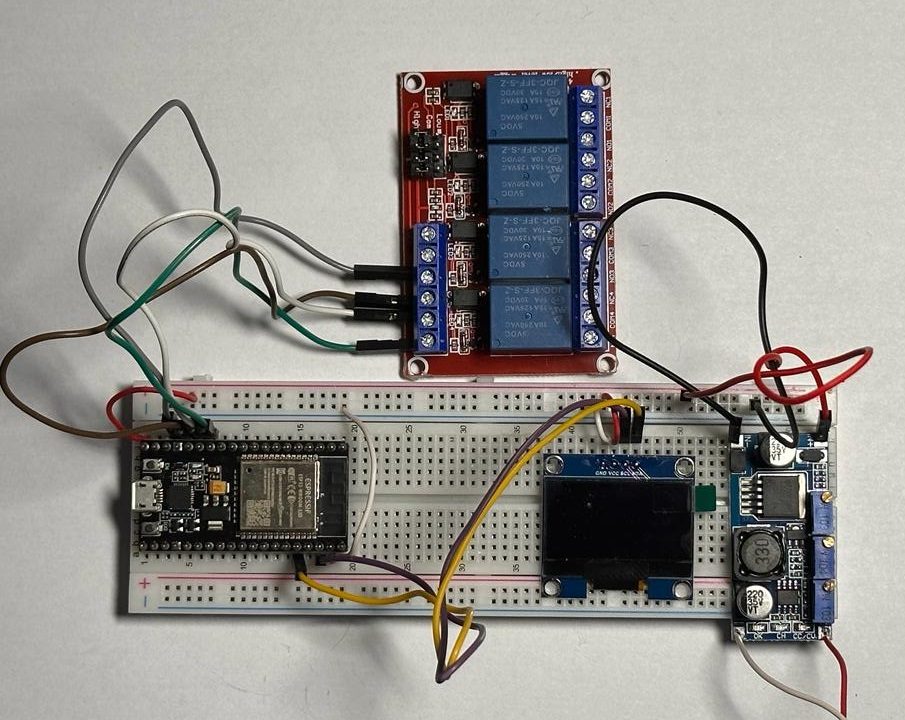
\includegraphics[width=1\textwidth]{./Figures/control_riego2.jpg}
		\caption[Conexionado]{Conexionado.}
		\label{fig:riego2}
     \end{subfigure}
      \begin{subfigure}[b]{0.45\textwidth}
	\centering
		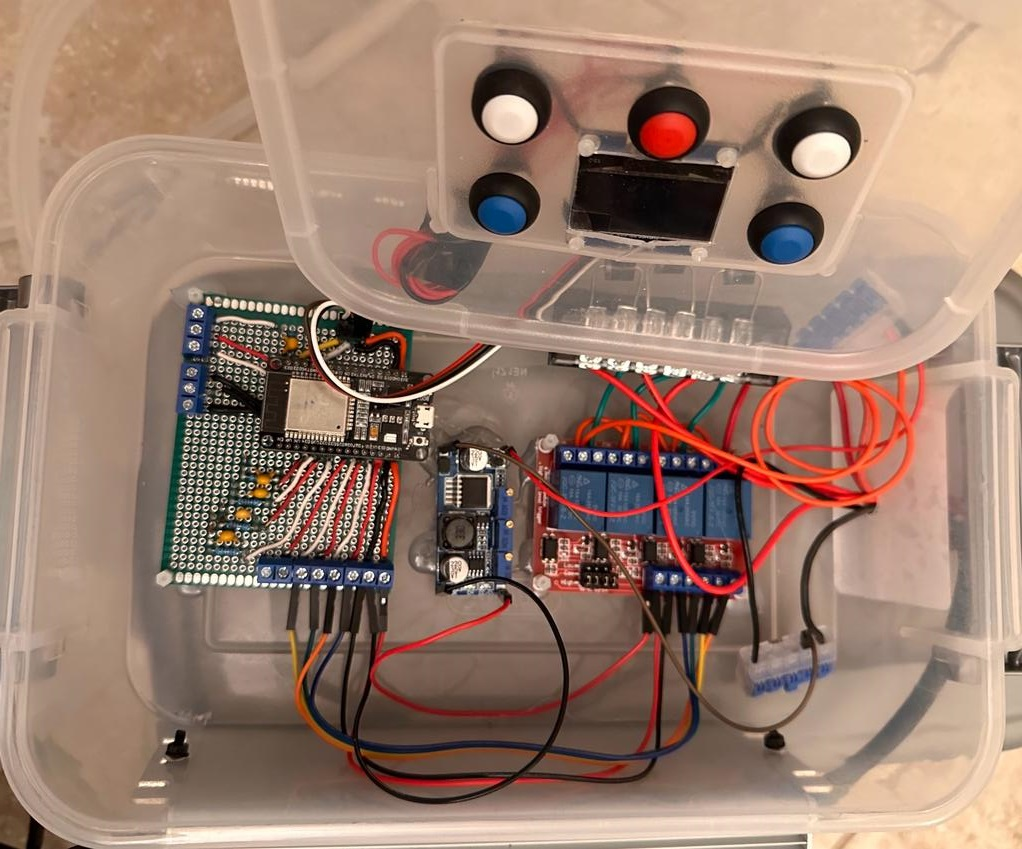
\includegraphics[width=0.8\textwidth]{./Figures/control_riego3.jpg}
		\caption[Conexionado]{Módulo finalizado en su caja protectora.}
		\label{fig:riego3}
     \end{subfigure}	
%			\begin{subfigure}[b]{0.45\textwidth}
%	\centering
%		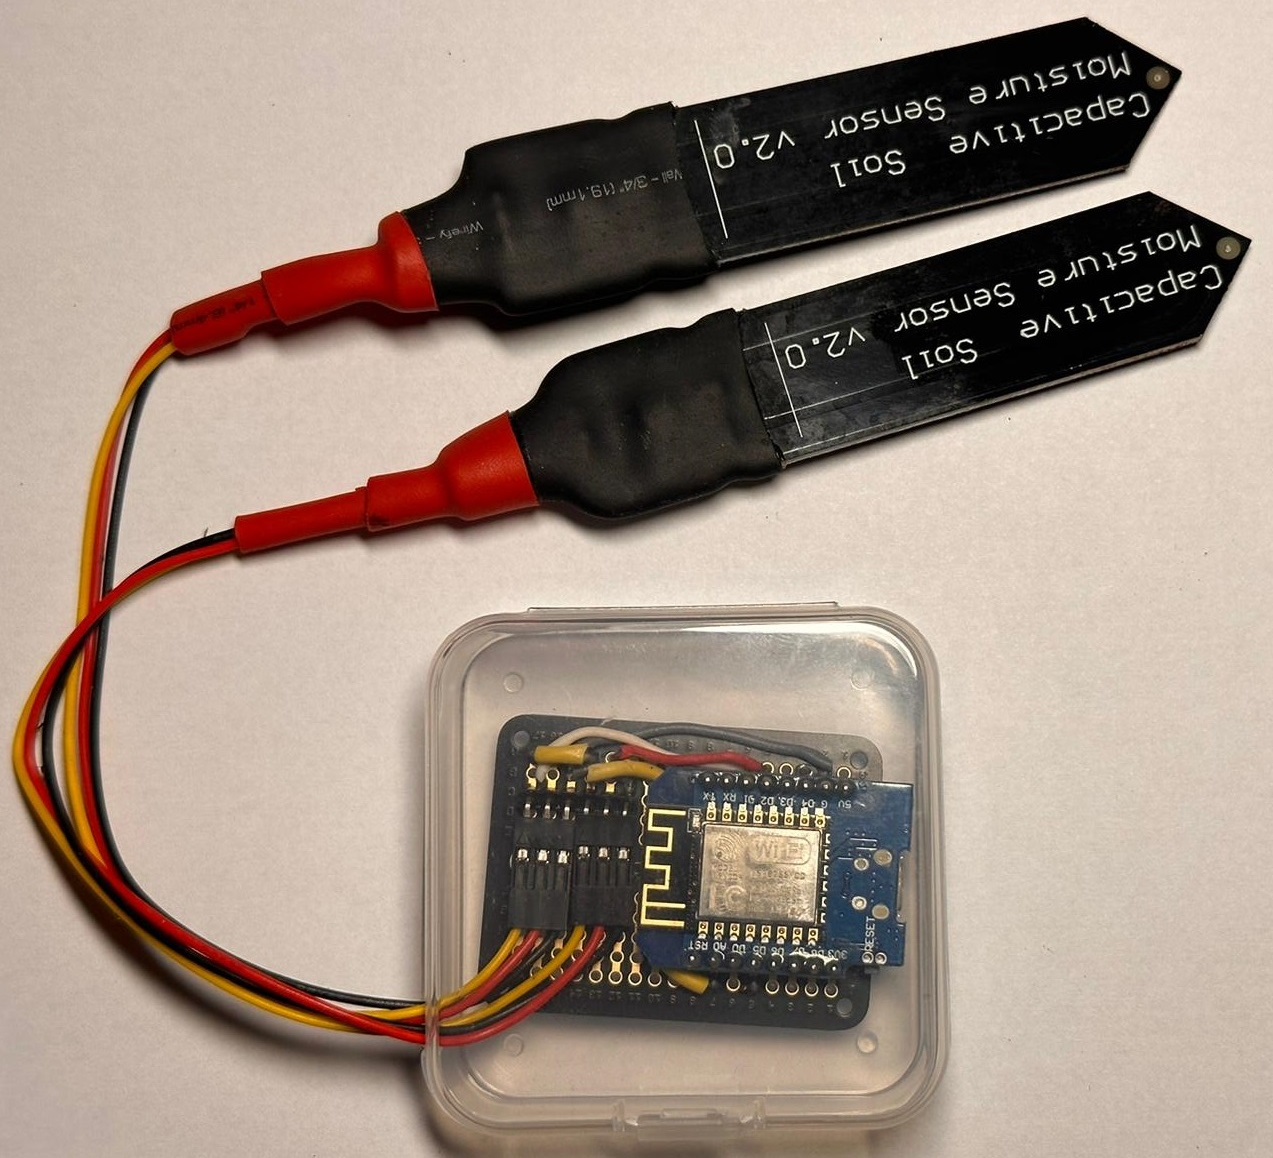
\includegraphics[width=0.60\textwidth]{./Figures/soil3.jpg}
%		\caption[Módulo en su caja protectora]{Módulo en su caja protectora.}
%		\label{fig:soil4}
%     \end{subfigure}
     \hfill
        \caption[Módulo de control de riego]{Módulo de control de riego.}
        \label{fig:riego_control}
\end{figure}


%\begin{figure}[!h]
%	\centering
%	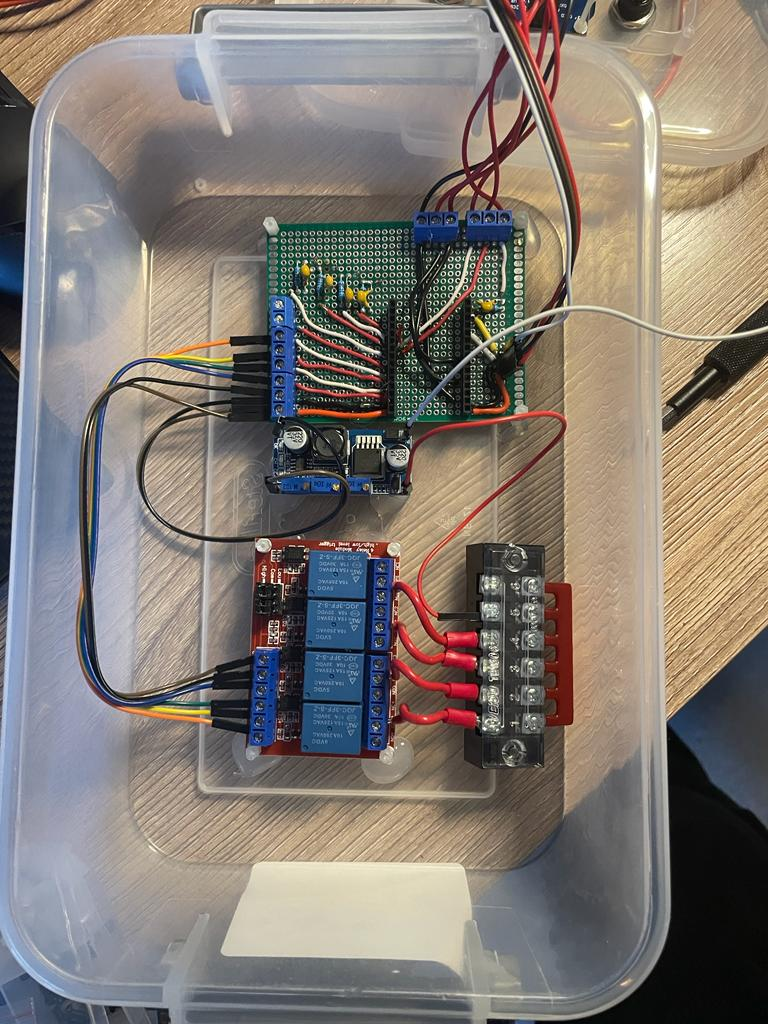
\includegraphics[width=0.5\textwidth]{./Figures/riego1.jpg}
%	\caption[Módulo completo en su caja protectora]{Módulo completo en su caja protectora.}
%	\label{fig:riego_control}
%\end{figure}
 
\pagebreak

\subsection{Módulo sensor de temperatura y humedad}
\label{Módulo sensor de temperatura y humedad}

Está compuesto por un microcontrolador ESP8266, un sensor DHT22 y una pantalla LCD/OLED SSH1106 para visualizar los valores de temperatura y humedad  \textit{in situ} en tiempo real. El esquema de conexión de los componentes se puede ver en la figura \ref{fig:tempschem}.

A diferencia de las sondas de humedad del suelo, el sensor de temperatura y humedad está pensado para instalarse en una ubicación fija 
con acceso a la red eléctrica. Por este motivo no se consideró configurarlo para soportar \textit{deep sleep}.



La construcción del módulo se realizó sobre placa PCB experimental en forma similar a los demás sistemas.
Para proteger los componentes se utilizó una caja de polipropileno transparente. El sensor DHT22 quedó expuesto para medir las condiciones ambientales como muestra la figura \ref{fig:temp_sensor}.


\begin{figure}[!h]
	\centering
	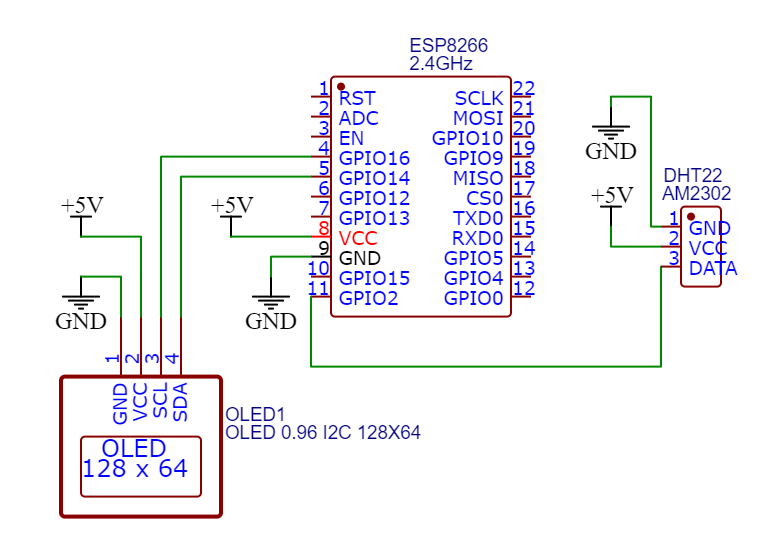
\includegraphics[width=0.7\textwidth]{./Figures/temp_sensor.png}
	\caption[Conexión del sensor de temperatura y humedad]{Conexión del sensor de temperatura y humedad.}
	\label{fig:tempschem}
\end{figure}


\begin{figure}[!h]
	\centering
	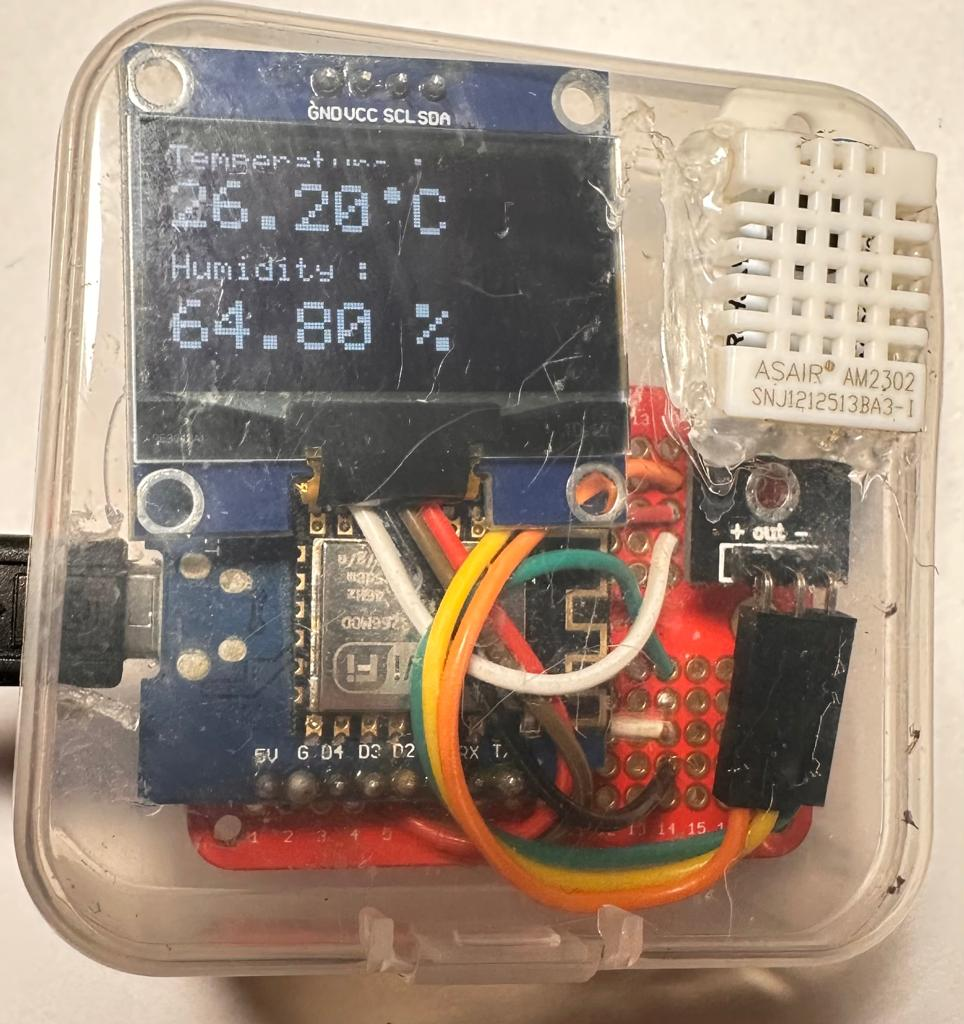
\includegraphics[width=0.5\textwidth]{./Figures/sensor_temp.jpg}
	\caption[Módulo completo en su caja protectora]{Módulo completo en su caja protectora.}
	\label{fig:temp_sensor}
\end{figure}


\subsection{Módulo controlador de clima}
\label{Módulo controlador de clima}

Es el responsable de accionar los ventiladores en el invernadero. Para el diseño se utilizó un chip ESP8266 conectado a un relé de una vía como se muestra en la figura \ref{fig:ventschem}. 

Dado que la salida del microcontrolador es de 3,3 V para el prototipo se seleccionó un relé que pueda ser accionado con ese valor de tensión, para evitar el uso de componentes adicionales tal como un convertidor de tensión DC-DC \textit{step up}. 

En la figura \ref{fig:ventcontrol} se ilustra el proceso de construcción del módulo. 



\begin{figure}[!h]
	\centering
	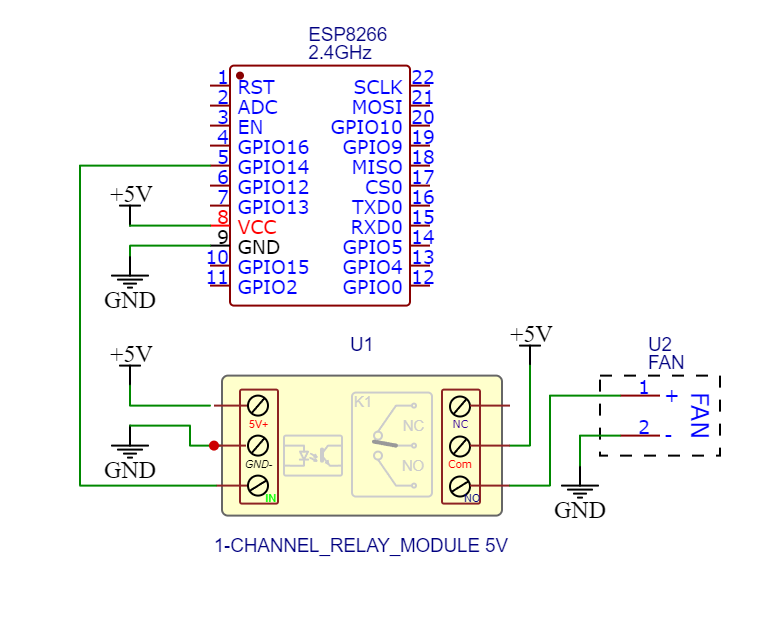
\includegraphics[width=0.7\textwidth]{./Figures/vent_schem.png}
	\caption[Conexión del módulo de control de clima]{Conexión del módulo de control de clima.}
	\label{fig:ventschem}
\end{figure}


\begin{figure}[!htpb]
     \centering
     \begin{subfigure}[b]{0.45\textwidth}
		\centering
		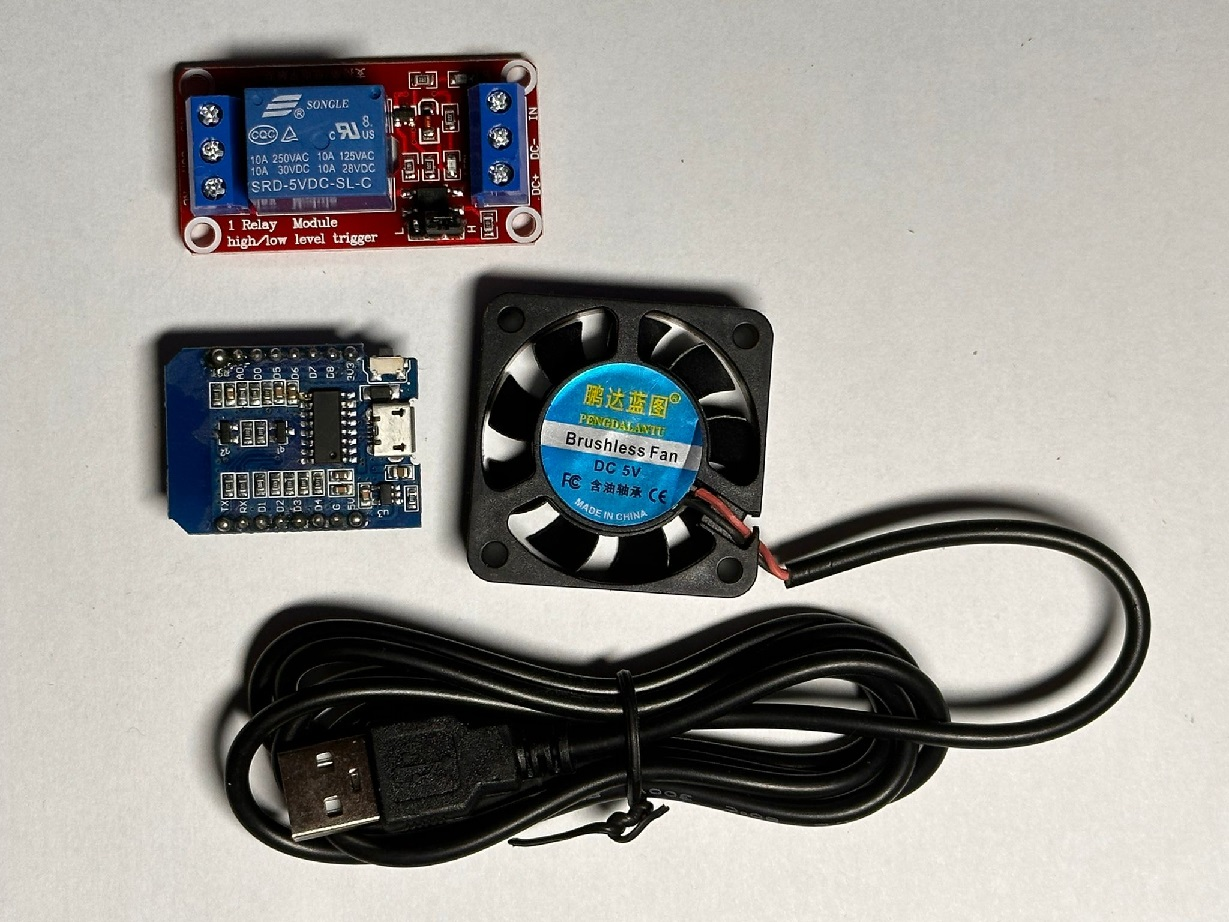
\includegraphics[width=0.80\textwidth]{./Figures/vent_control.jpg}
		\caption{Detalle de los componentes.}
		\label{fig:vent1}
     \end{subfigure}
     \hfill
     \begin{subfigure}[b]{0.45\textwidth}
	\centering
		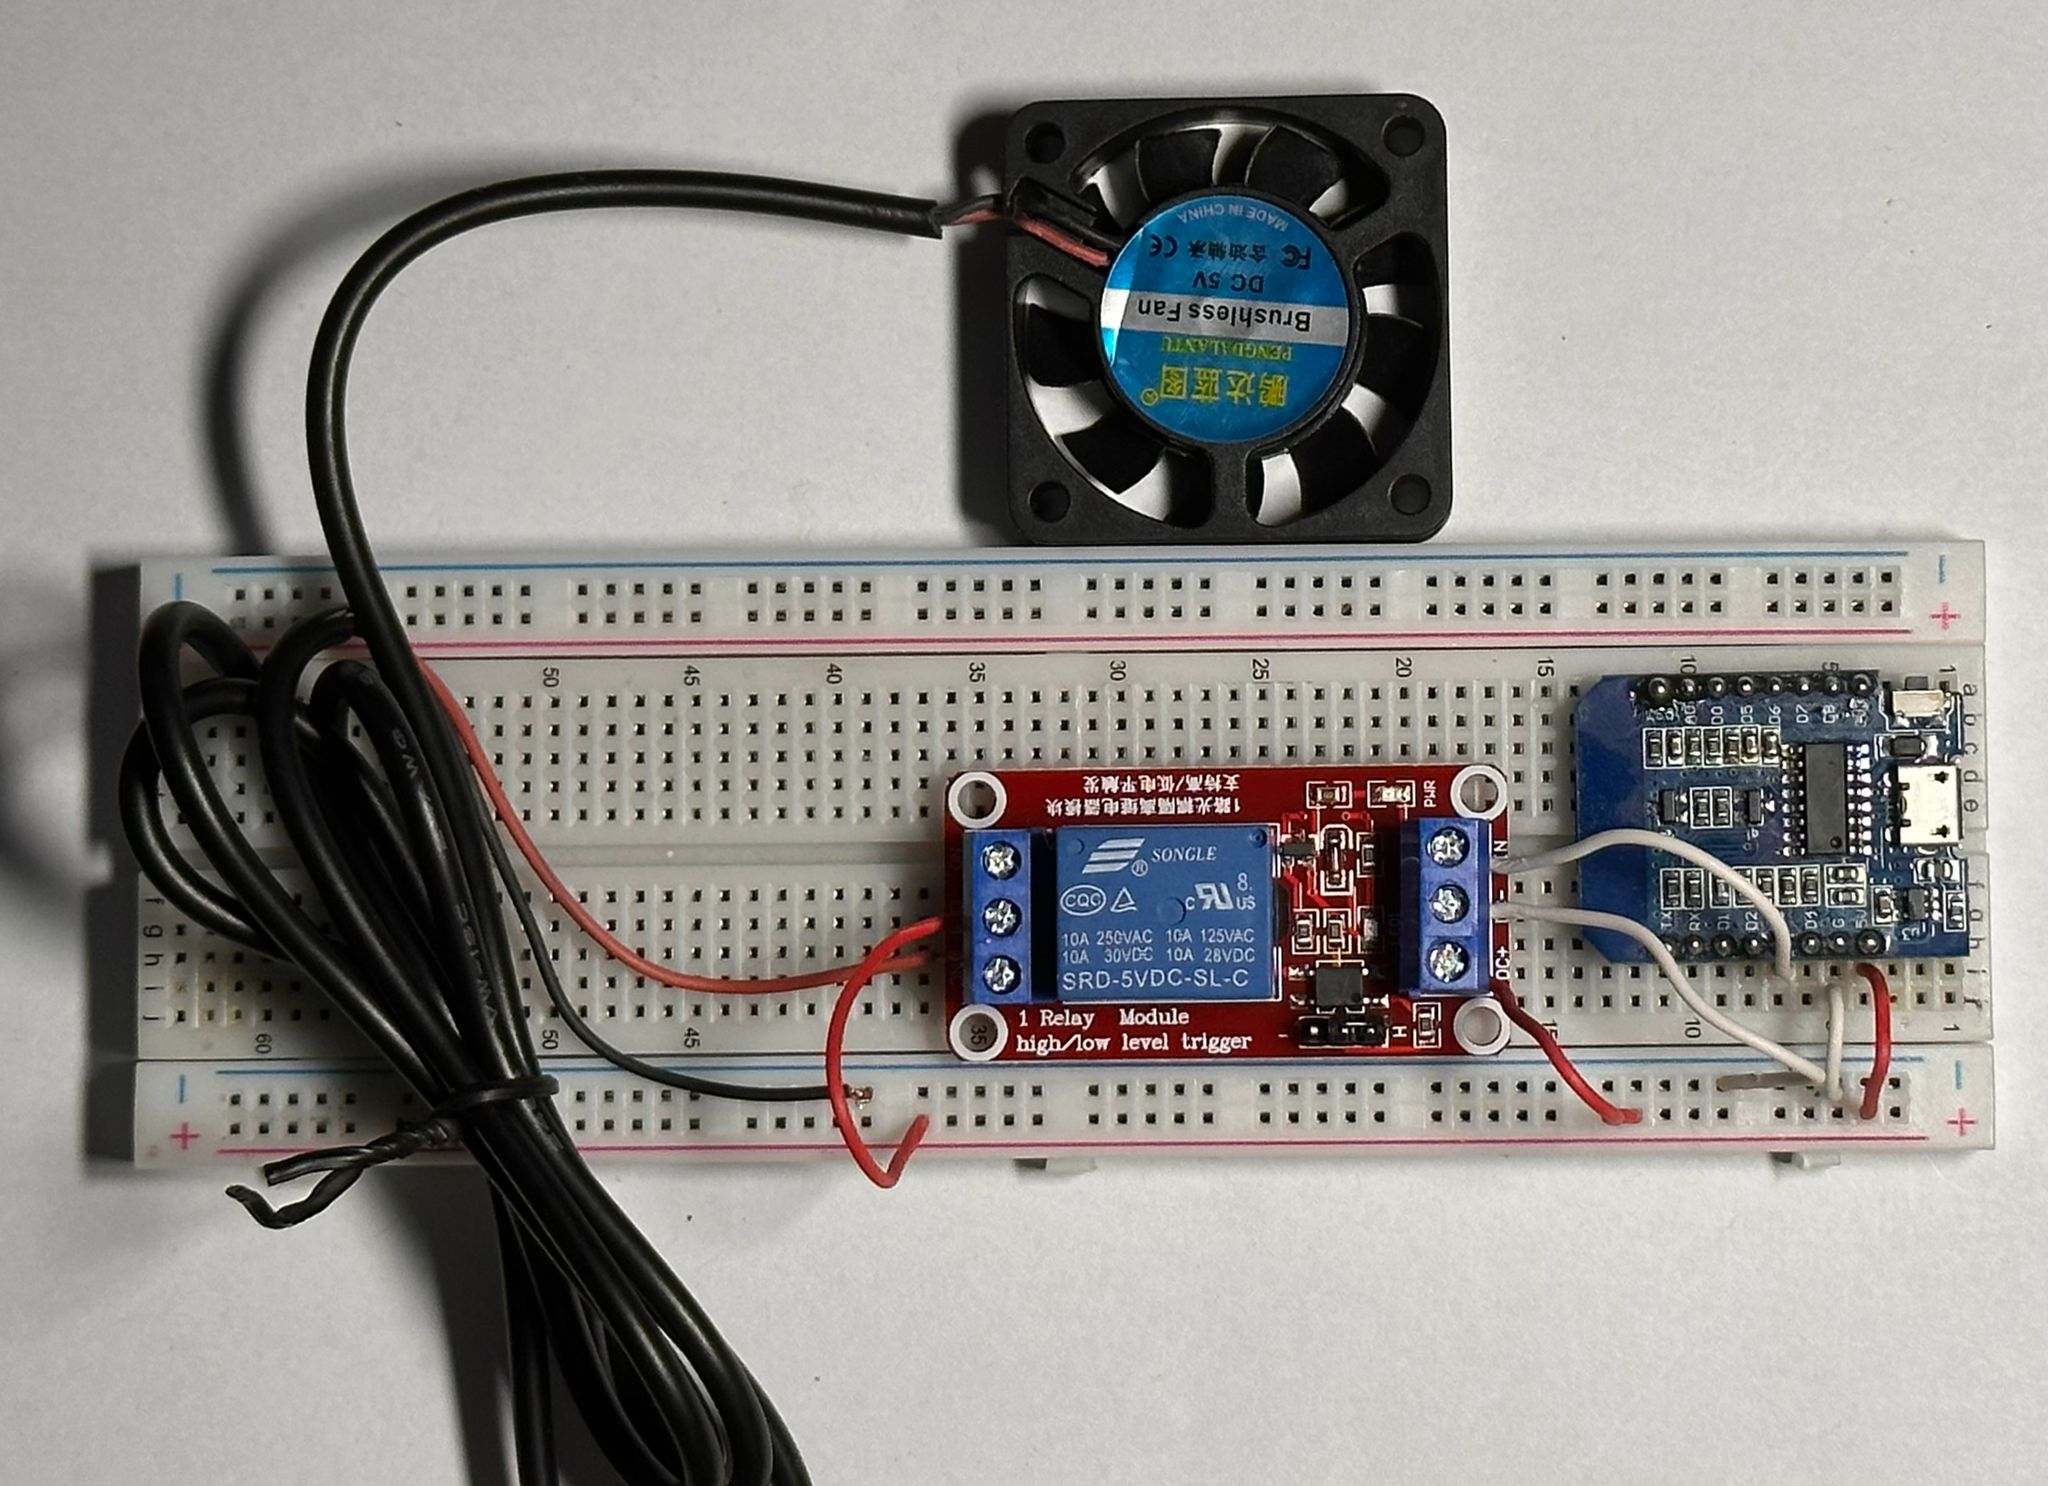
\includegraphics[width=0.80\textwidth]{./Figures/vent_proto.jpg}
		\caption{Conexionado.}
		\label{fig:vent2}
     \end{subfigure}	
	\begin{subfigure}[b]{0.45\textwidth}
		\centering
		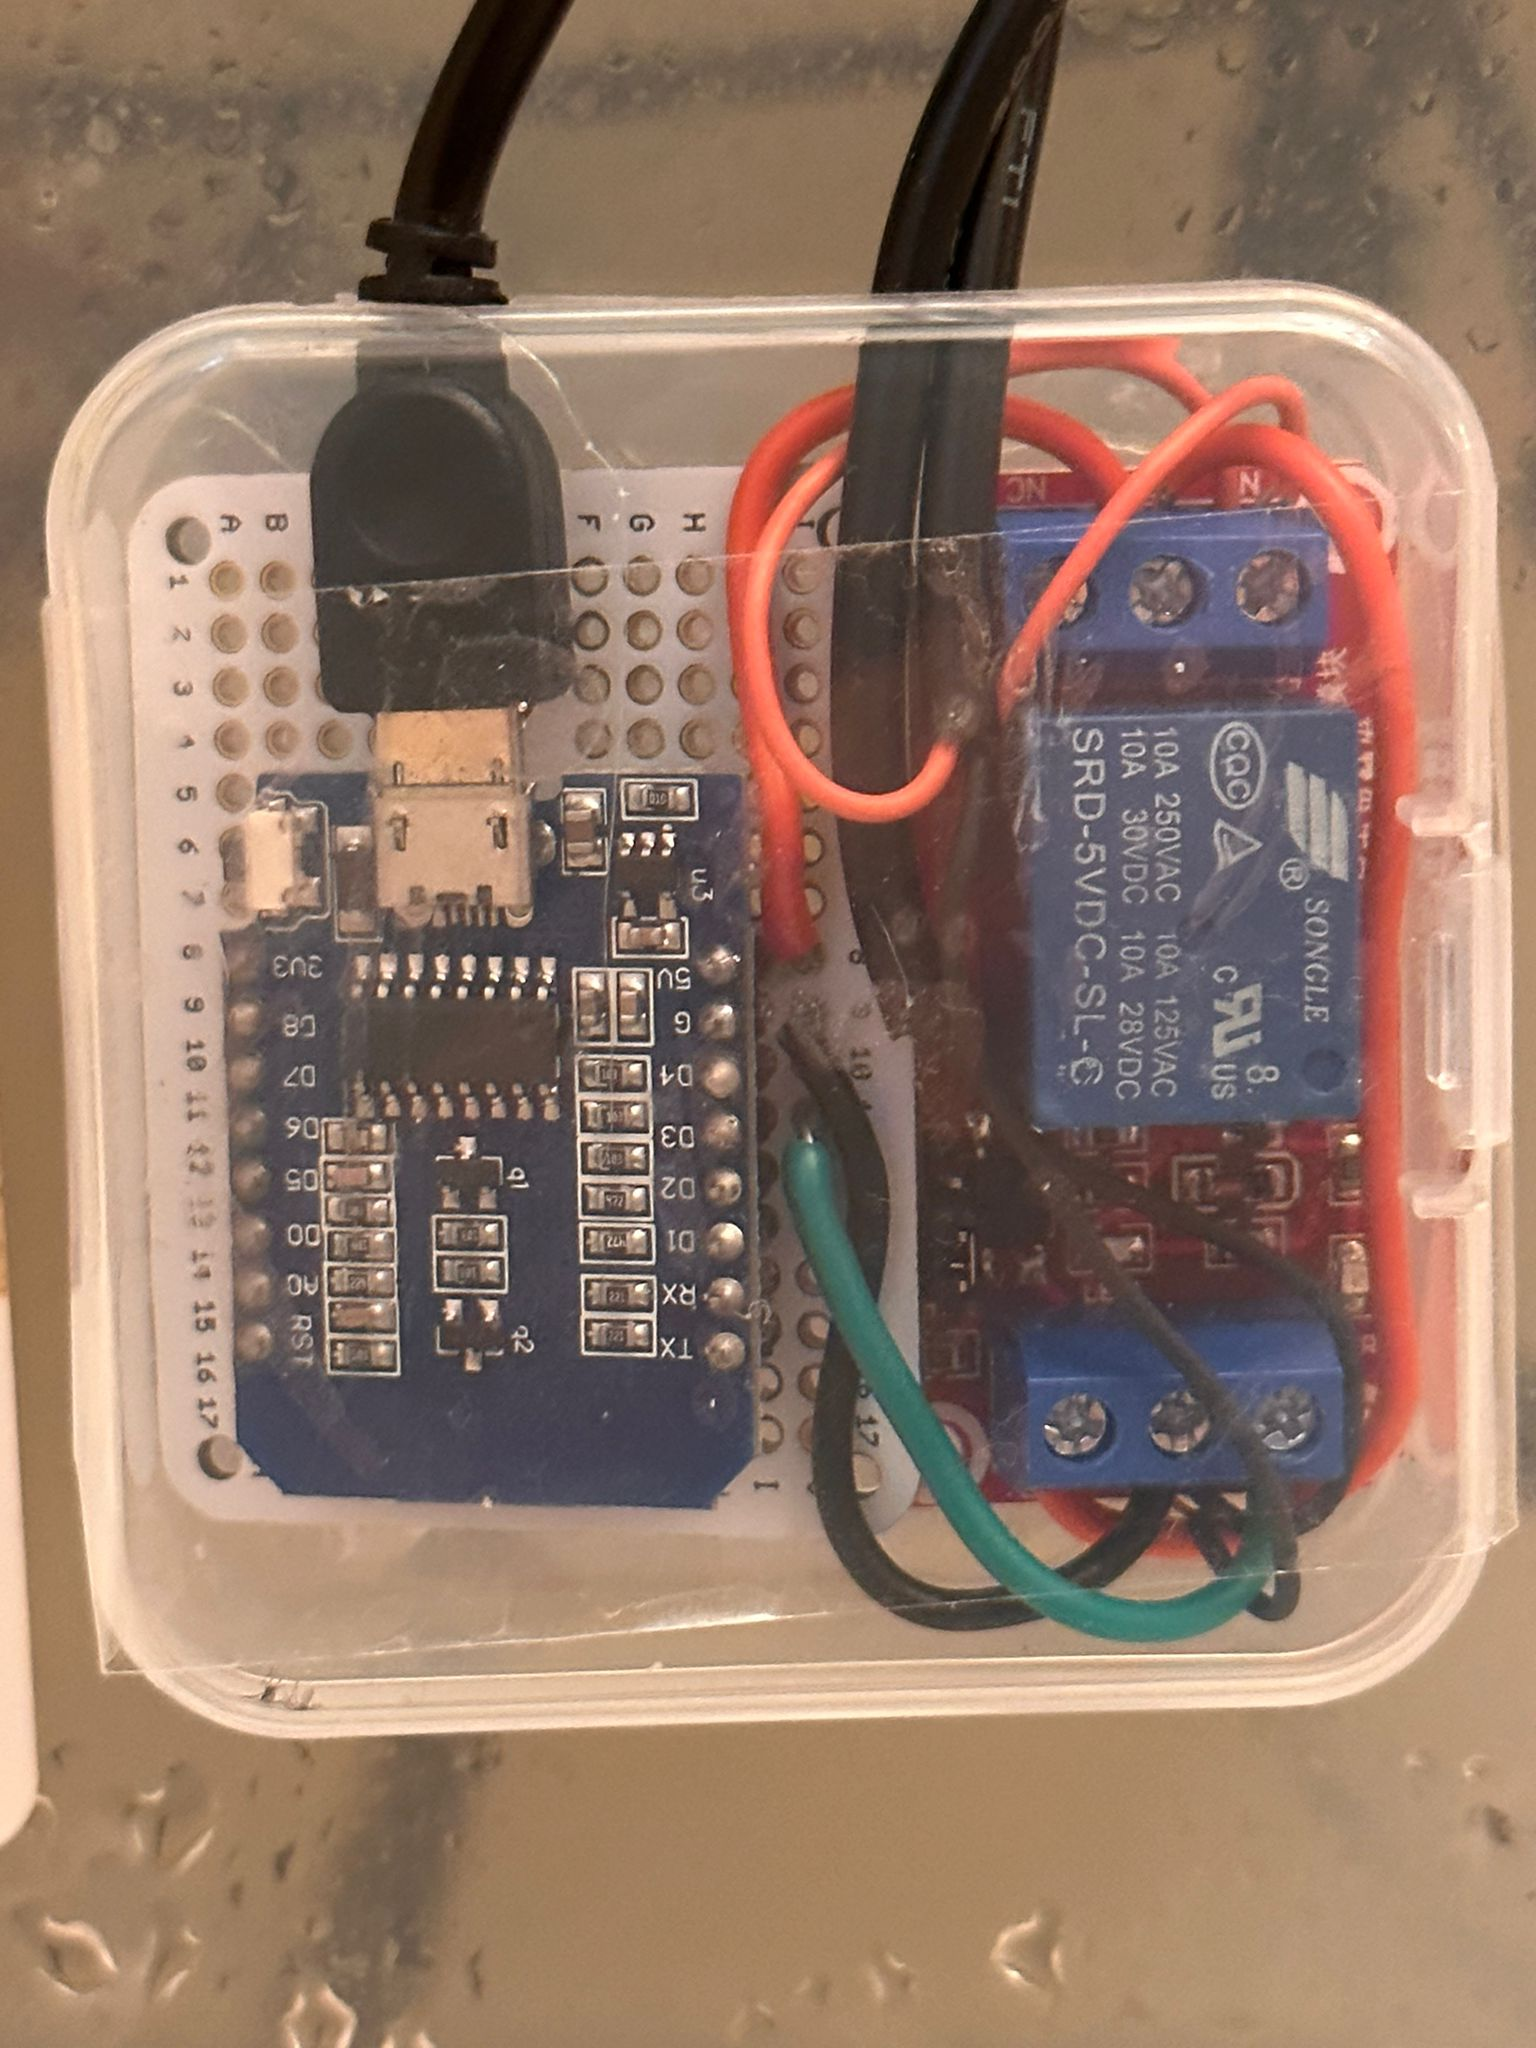
\includegraphics[width=0.60\textwidth]{./Figures/vent_assembled.jpg}
		\caption{Módulo finalizado en su caja protectora.}
		\label{fig:vent3}
     \end{subfigure}
     \hfill
        \caption[Módulo de control de clima]{Módulo de control de clima.}
        \label{fig:ventcontrol}
\end{figure}


\pagebreak

\section{Desarrollo del firmware}
\label{sec:Desarrollo del firmware}

Como el soporte y la expansión del sistema quedará a cargo del cliente, se optó por desarrollar el firmware en C++ mediante la aplicación Arduino IDE. Esta elección se fundamenta en la baja curva de aprendizaje de la herramienta, la amplia disponibilidad de librerías y ejemplos para el uso de componentes, además de contar con una vasta comunidad de entusiastas de IoT en Internet.

En líneas generales, un programa escrito mediante esta herramienta respeta una estructura de dos bloques:

\begin{enumerate}

\item Setup: función que se ejecuta una única vez al comienzo del programa y se utiliza para inicializar las variables, configurar los pines de entrada y salida y establecer las comunicaciones necesarias, tales como la velocidad del puerto serial o la conexión a la red Wi-Fi.

\item Loop: función que se ejecuta continuamente en un bucle que, por lo general, solo se interrumpe al apagar el dispositivo. En esta sección se encuentra el código principal del firmware.
\end{enumerate}
Adicionalmente, el código puede contener variables, funciones y bibliotecas.

Para facilitar la conexión a la aplicación ThingsBoard se utilizó el kit de desarrollo Arduino ThingsBoard SDK \citep{tbsdk} que, entre otras funciones, provee mecanismos para el manejo de los protocolos MQTT y RPC, a la vez que permite la actualización OTA \citep{8999425} del firmware.

Desde el mismo Arduino IDE se transfiere el código generado a la memoria no volátil (\textit{flash}) del dispositivo. Al iniciar (o reiniciar) el microcontrolador, el programa se carga desde la memoria \textit{flash} a la memoria RAM y comienza su ejecución.



\subsection{Módulos sensores de humedad del suelo}
\label{Módulos sensores de humedad del suelo}



En este caso, debido a que ThingsBoard no permite ajustar los períodos de retención de las colas de MQTT para soportar configuraciones prolongadas de \textit{deep sleep}, se resolvió utilizar el protocolo HTTP para las comunicaciones entre el módulo y la aplicación central. 

Luego del inicio, el programa realiza una llamada HTTP para obtener el valor del tiempo de hibernación y a continuación lleva a cabo la lectura de los sensores según el caso:
\begin{itemize}
\item Sensor simple: lee el valor del pin de conversión analógica a digital (ADC).
\item Sensor doble: como el chip ESP8266 posee un único pin ADC compartido por ambas sondas, se procede al energizado secuencial de los sensores al activar la salida GPIO correspondiente, como se mostró en la figura \ref{fig:soilschem2}. 

\end{itemize}


Para que el módulo pueda reportar un medición que represente la humedad del suelo, es necesario llevar a cabo una conversión del valor leído en el pin ADC. La relación entre cuentas valor obtenido y humedad se obtiene con una variante respecto del método descrito por Joshua Hrisko \citep{soilcalibration} que consiste en realizar mediciones en suelo seco para luego ir agregando cantidades precisas de agua sobre las que se evalúa la diferencia de potencial observada en cada caso. Del proceso resulta una expresión que permite estimar el contenido volumétrico de agua presente.

Una vez obtenido el o los valores, se los reporta a la aplicación por medio de una llamada HTTP POST y se da inicio al período de \textit{deep sleep} durante el lapso de tiempo establecido.

El flujo de ejecución del código para un módulo doble se visualiza en la figura \ref{fig:flow_soilsensor}.


\begin{figure}[!h]
	\centering
	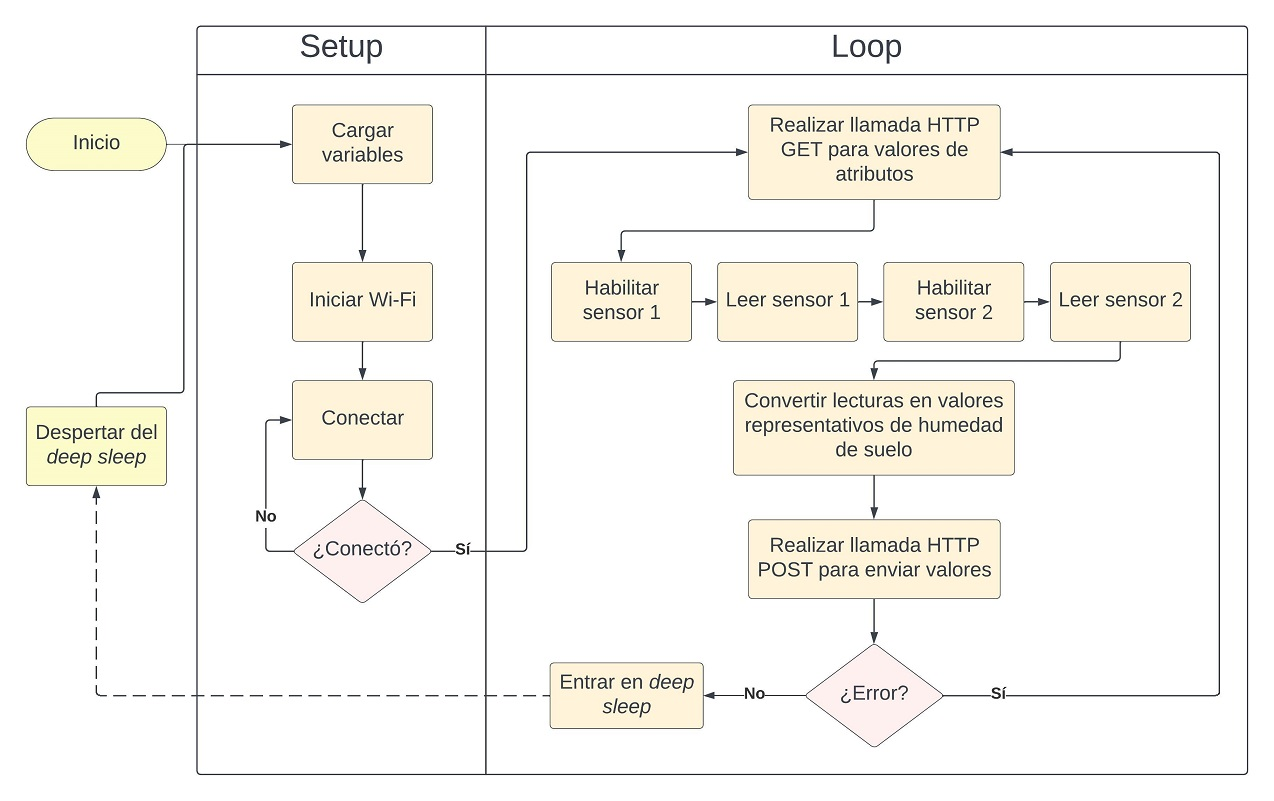
\includegraphics[width=1\textwidth]{./Figures/chapter3/FirmwareSoilSensor.jpg}
	\caption[Diagrama de flujo del firmware de los módulos sensores de humedad del suelo]{Diagrama de flujo del firmware de los módulos sensores de humedad del suelo.}
	\label{fig:flow_soilsensor}
\end{figure}



\subsection{Módulo controlador del riego}
\label{Módulo controlador del riego}

Es el módulo de mayor complejidad, tal como se refleja en las figuras \ref{fig:flow_riegocontrol}, \ref{fig:flow_valvecontrol}  y \ref{fig:flow_bombacontrol}.

\begin{figure}[!h]
	\centering
	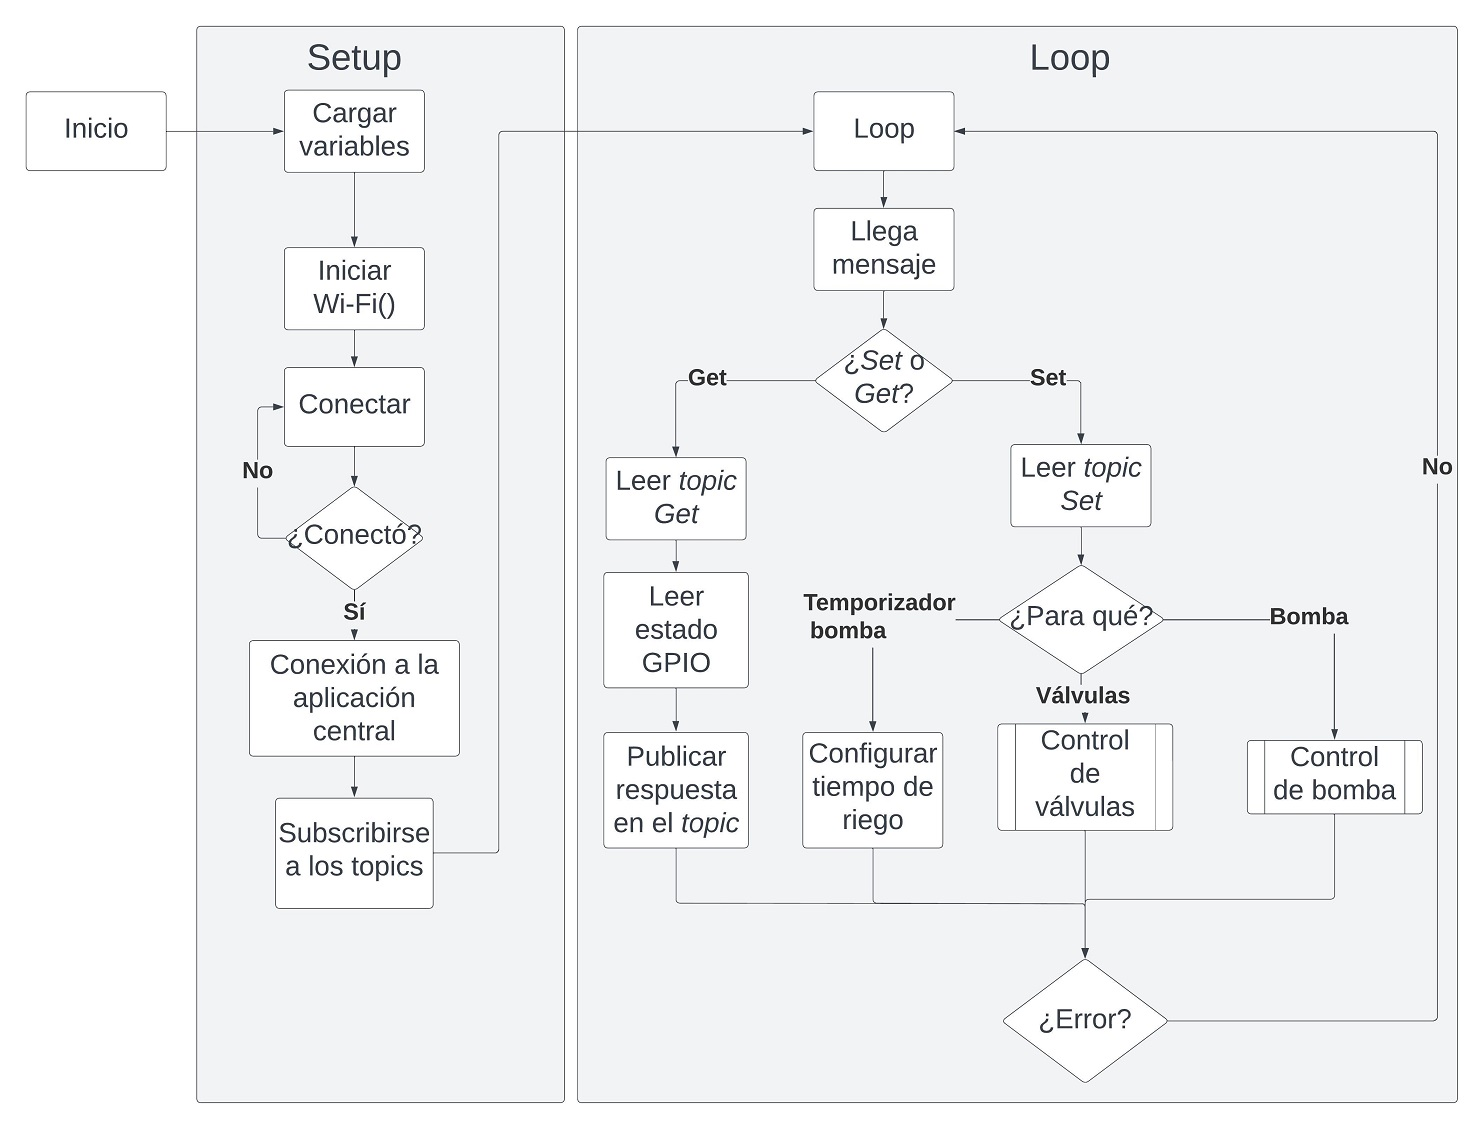
\includegraphics[width=1.0\textwidth]{./Figures/chapter3/FirmwareRiegoControl.jpg}
	\caption[Diagrama de flujo del firmware del módulo de control de riego]{Diagrama de flujo del firmware del módulo de control de riego.}
	\label{fig:flow_riegocontrol}
\end{figure}
%
%\begin{tikzpicture}[node distance=2cm]
%
%\node (start) [startstop] {Inicio};
%\node (pro1a) [process, right of=start, xshift= 1cm] {Cargar variables};
%\node (pro1b) [process, below of=pro1a, yshift= -0.5cm] {Iniciar Wi-Fi};
%\node (pro1c) [process, below of=pro1b, yshift= -0.5cm] {Conectar};
%\node (dec1) [decision, below of=pro1c, yshift=-0.5cm] {¿Conectó?};
%\node (pro1d) [process, below of=dec1, yshift= -0.5cm] {Conexión a la aplicación central};
%\node (pro1e) [process, below of=pro1d, yshift= -0.5cm] {Suscribirse a los \textit{topics}};
%
%
%%\node (pro2a) [process, below left of=dec1, xshift=-2cm] {Step 2a};
%%\node (pro2b) [process, below right of=dec1, xshift=2cm] {Step 2b};
%%\node (dec2) [decision, below of=pro2a, yshift=-1cm] {Decision 2};
%%\node (pro3a) [process, below left of=dec2, xshift=-2cm] {Step 3a};
%%\node (pro3b) [process, below right of=dec2, xshift=2cm] {Step 3b};
%\node (stop) [startstop, below of=pro3a] {Stop};
%
%\draw [arrow] (start) -- (pro1a);
%\draw [arrow] (pro1a) -- (pro1b);
%\draw [arrow] (pro1b) -- (pro1c);
%\draw [arrow] (pro1c) -- (dec1);
%\draw [arrow] (dec1) -| node[anchor=south] {sí} (pro1d);
%\draw [arrow] (dec1) -| node[anchor=north] {no} (pro1c);
%\draw [arrow] (pro1d) -- (pro1e);
%%\draw [arrow] (pro2a) -- (dec2);
%\draw [arrow] (pro2b) -- (dec2);
%\draw [arrow] (dec2) -| node[anchor=north west] {yes} (pro3a);
%\draw [arrow] (dec2) -| node[anchor=north east] {no} (pro3b);
%\draw [arrow] (pro3a) -- (stop);
%\draw [arrow] (pro3b) -- (stop);
%
%\end{tikzpicture}




La ejecución inicia con la carga de variables, entre las que se destacan:
\begin{itemize}
\item Tiempo de riego: define la duración de encendido de la bomba en segundos.
\item Bomba lista: variable lógica que indica el pedido de encendido de la bomba.
\item Estado de válvulas: controlan las GPIOs de las válvulas.
\item Estado de bomba: controla la GPIO de la bomba.
\end{itemize}

Luego de la conexión a la red Wi-Fi, el firmware se registra con la aplicación y se suscribe a los \textit{getter} y \textit{setter topics} para reportar los estados a la aplicación o recibir comandos.



En el caso de recibir un mensaje de pedido de información, el código reporta el o los valores de las variables solicitadas en el \textit{topic} de respuesta. Por otro lado, si el mensaje recibido indica realizar un cambio de estado, se pueden presentar las siguientes situaciones:
\pagebreak

\begin{itemize}
\item Pedido de reconfigurar el tiempo de riego: el código actualiza la variable y reinicia el bucle.

\item Pedido de apertura o cierre de válvula:
    \begin{itemize}
    \item Apertura: procede a abrir la válvula seleccionada y  comprueba si la bomba se encuentra en estado de pedido de encendido (bomba lista), en cuyo caso ordena el encendido.
    \item Cierre: verifica si otras válvulas están abiertas y en caso afirmativo procede con el cierre. En caso contrario, si es la única, ordena el apagado de la bomba y luego el cierre de la válvula.
    
    \end{itemize}

\item Pedido de encendido o apagado de la bomba:
    \begin{itemize}
    \item Encendido: en el caso de haber al menos una válvula abierta, procede a encender la bomba durante el tiempo que indique la variable de duración de riego. Una vez finalizado, procede ordenadamente al apagado de la bomba y al cierre de las válvulas. De no haber válvulas abiertas, se configura la variable de bomba lista en positivo, indicando que el riego fue pedido pero aún no están dadas las condiciones para habilitarlo.
    \item Apagado: en el caso de requerir una interrupción en el riego, se ordena el apagado de la bomba y el cierre de las válvulas.
    
    \end{itemize}



\end{itemize}




\begin{figure}[!h]
	\centering
	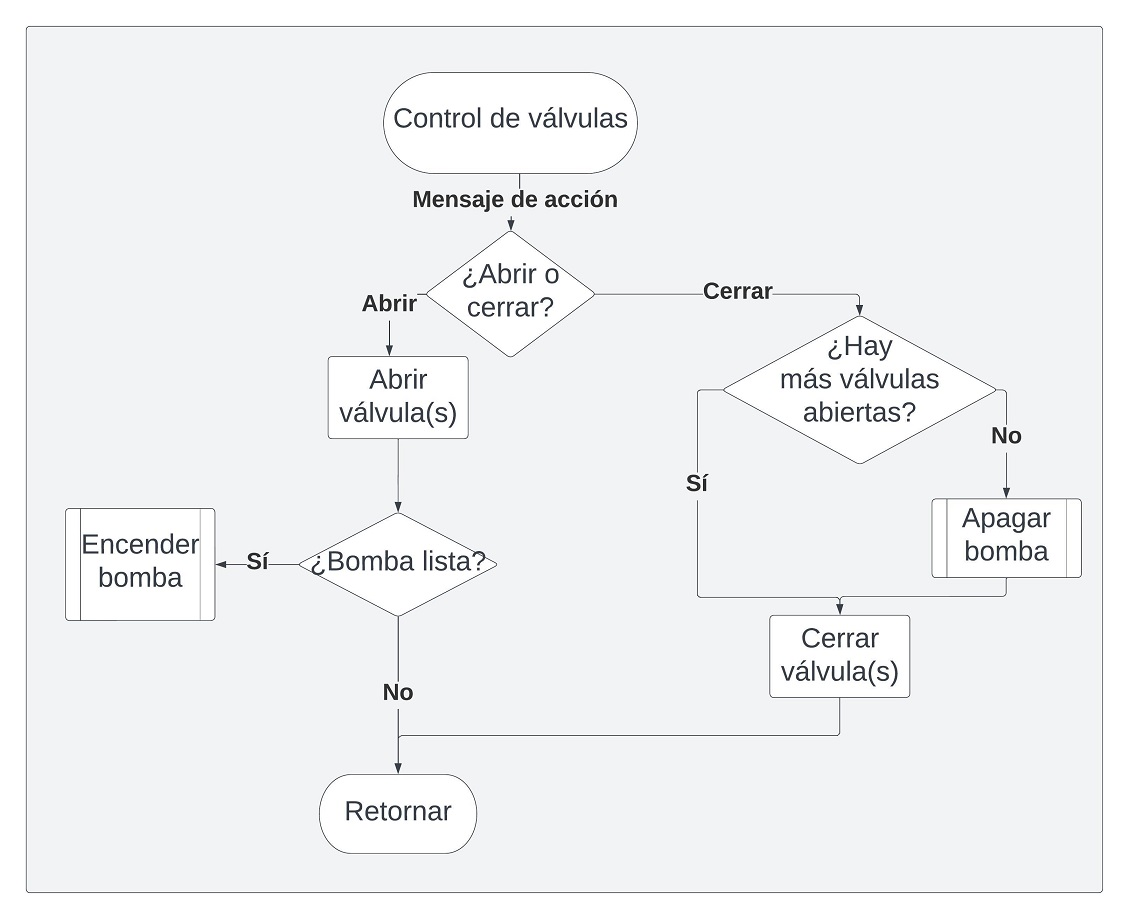
\includegraphics[width=0.7\textwidth]{./Figures/chapter3/FirmwareValveControl.jpg}
	\caption[Diagrama de flujo del firmware del módulo de control de riego - control de válvulas]{Diagrama de flujo del firmware del módulo de control de riego - control de válvulas.}
	\label{fig:flow_valvecontrol}
\end{figure}

\begin{figure}[!h]
	\centering
	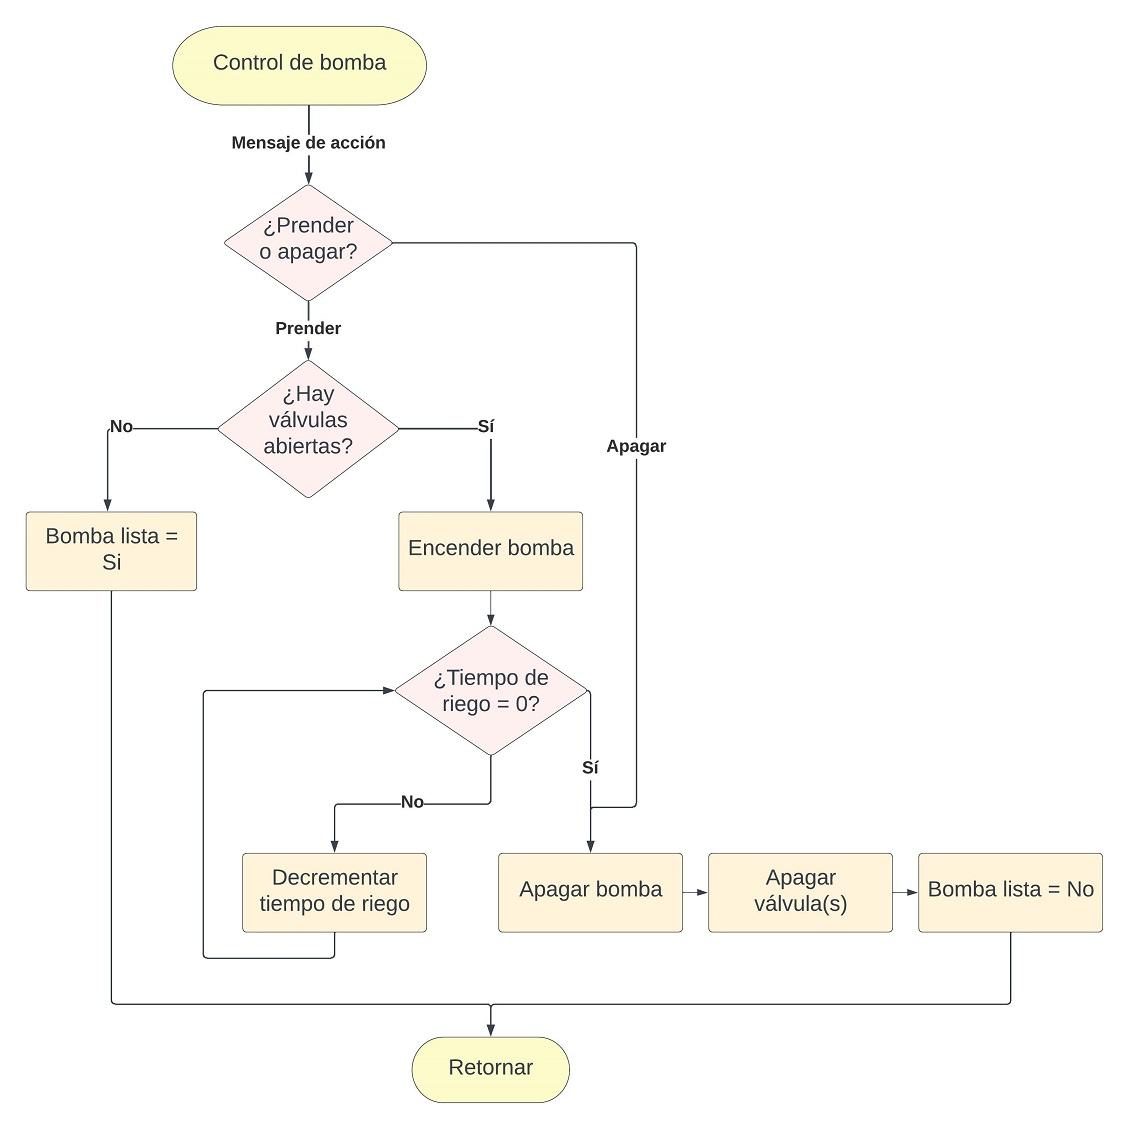
\includegraphics[width=0.8\textwidth]{./Figures/chapter3/FirmwarePumpControl.jpg}
	\caption[Diagrama de flujo del firmware del módulo de control de riego - control de bomba]{Diagrama de flujo del firmware del módulo de control de riego - control de bomba.}
	\label{fig:flow_bombacontrol}
\end{figure}







\pagebreak
\subsection{Módulo sensor de temperatura y humedad}
\label{Módulo sensor de temperatura y humedad}

La figura \ref{fig:flow_tempsensor} describe el funcionamiento de este módulo. Luego del ciclo de inicio y del setup, el código se encarga de obtener las medidas de temperatura y humedad, valores que despliega en la pantalla del módulo. Periódicamente estos valores se envían a la aplicación de acuerdo con un contador de ciclos. 


\begin{figure}[!h]
	\centering
	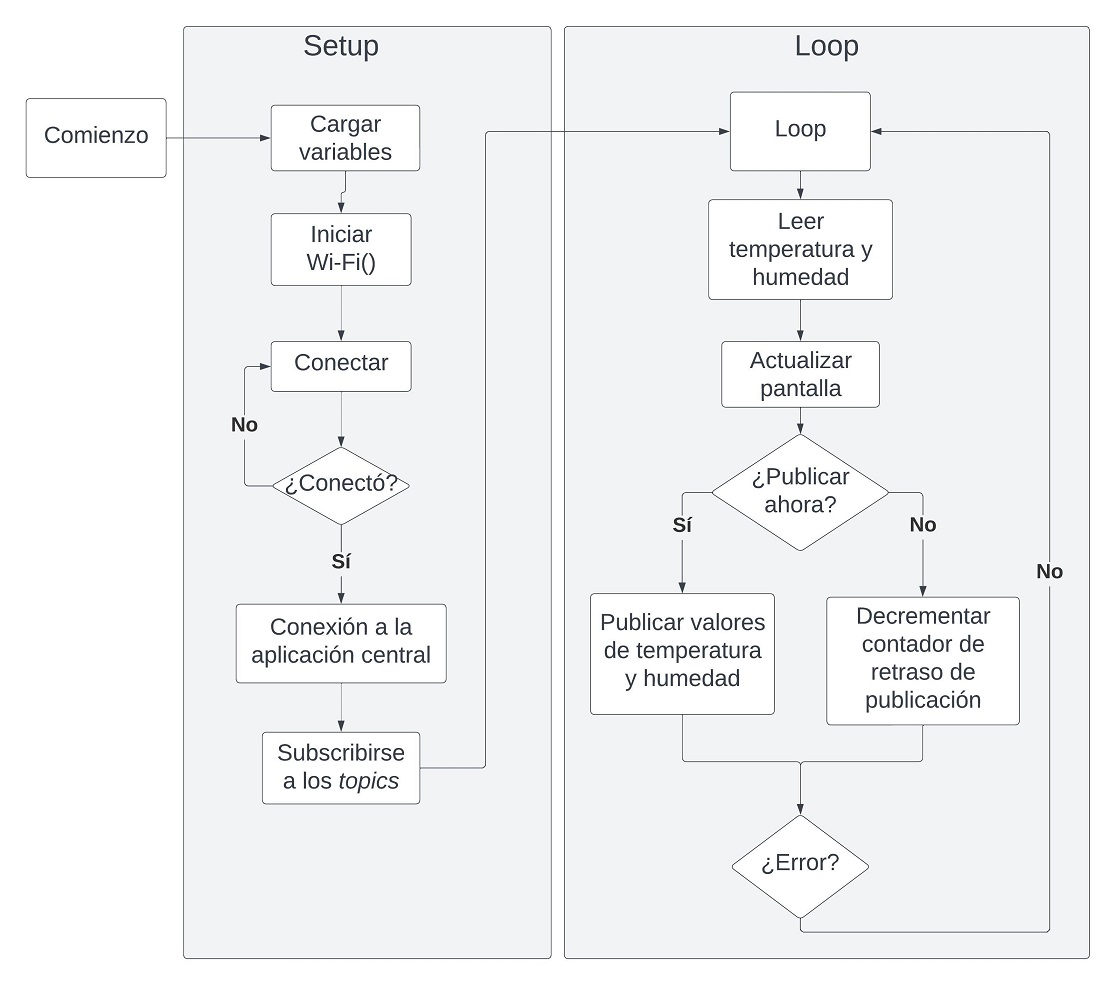
\includegraphics[width=0.9\textwidth]{./Figures/chapter3/FirmwareTempSensor.jpg}
	\caption[Diagrama de flujo del firmware del módulo sensor de temperatura y humedad]{Diagrama de flujo del firmware del módulo sensor de temperatura y humedad.}
	\label{fig:flow_tempsensor}
\end{figure}




\subsection{Módulo de control de clima}
\label{Módulo de control de clima}

Es el encargado del encendido y apagado de los ventiladores para controlar el clima.
Luego del inicio, el programa se conecta a la red, se subscribe en los \textit{topics} correspondientes e ingresa en la función de loop a la espera de mensajes. En caso de recibir un pedido de reporte, responde con el estado del pin GPIO asociado con el ventilador. Si recibe una orden de encendido o apagado, realiza la acción correspondiente y retorna al inicio del bucle.

En la figura \ref{fig:flow_climacontrol} se describe el flujo del código para este módulo.

\begin{figure}[!h]
	\centering
	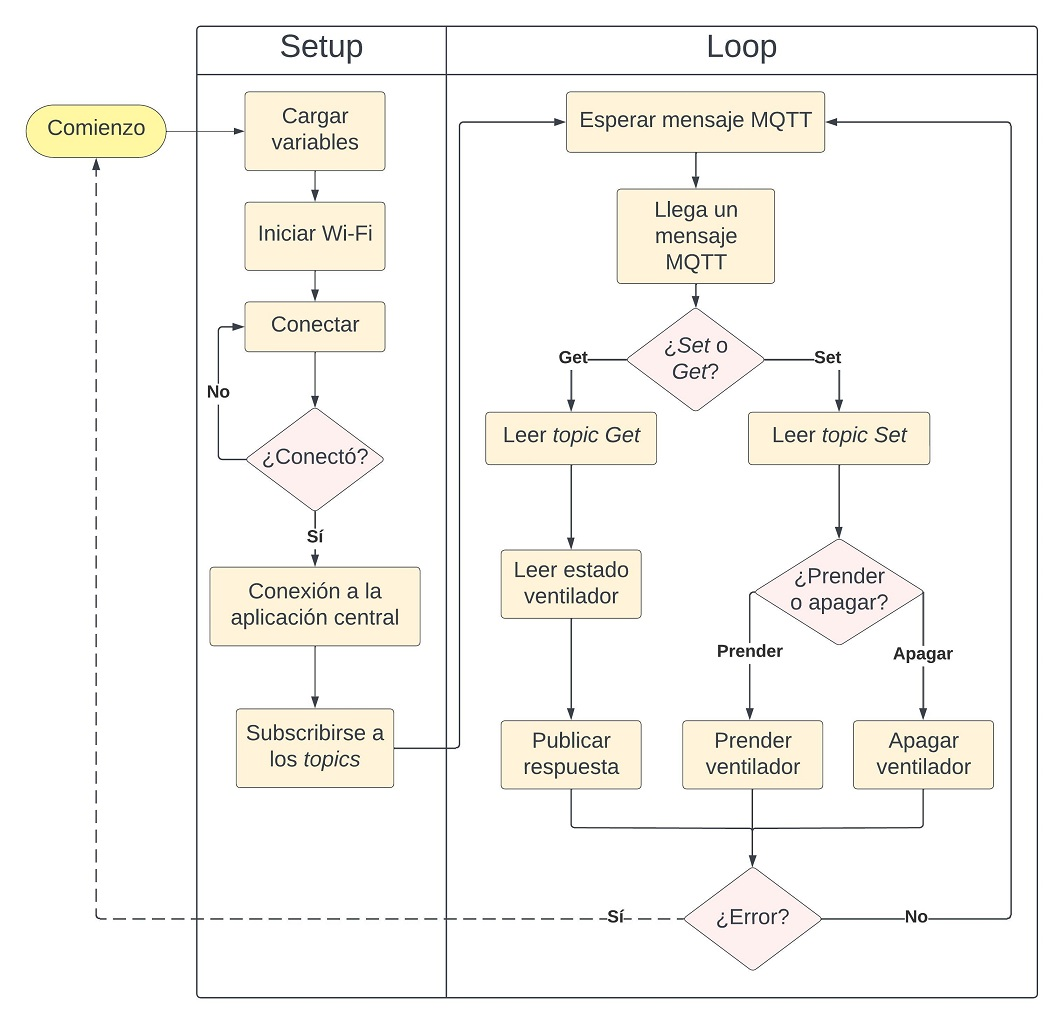
\includegraphics[width=0.9\textwidth]{./Figures/chapter3/FirmwareVentControl.jpg}
	\caption[Diagrama de flujo del firmware del módulo de control de clima]{Diagrama de flujo del firmware del módulo de control de clima.}
	\label{fig:flow_climacontrol}
\end{figure}









\section{Selección y configuración del software}
\label{sec:Selección y configuración del software}

La propiedad del cliente se encuentra en una zona rural con acceso a internet limitado, por tal motivo se implementó una solución local basada en  ThingsBoard Community Edition.
Esta plataforma tiene bajos requerimientos de hardware, buen diseño de seguridad y ofrece amplias posibilidades de expansión.

\subsection{Servidor de la aplicación}
\label{sec:Servidor de la aplicación}

La instalación se realizó sobre una Raspberry Pi 4B de 8 GB de memoria RAM, con sistema operativo Linux Raspbian versión 11, todo instalado sobre una tarjeta de memoria SD de 64 GB de capacidad.



\subsection{Configuración de la aplicación}
\label{sec:Configuración de la aplicación}

La instalación de la aplicación se realizó conforme a las instrucciones provistas por el desarrollador en su página oficial \citep{tb_install}.
ThingsBoard requiere de una base de datos para almacenar los valores de telemetría y atributos. Para una carga de hasta 5000 mensajes por segundo se recomienda el uso de PostgreSQL \citep{postgresql}. Dado que la cantidad de mensajes enviados es de aproximadamente 4 por minuto en el prototipo y no se espera un crecimiento desmedido en el pasaje a producción, la capacidad de memoria y procesamiento empleados resulta suficiente para la instalación conjunta de la base de datos y la aplicación.



\pagebreak
\subsection{Manejo de dispositivos}
\label{sec:Manejo de dispositivos}

La baja cardinalidad de módulos creados para el proyecto permitió emplear la interfaz web para gestionarlos en lugar de la opción programática mediante la API REST.
Al no contar con una CA para la generación de certificados, la autenticación de los dispositivos se resolvió mediante el empleo de tokens.

La figura \ref{fig:tb_devices3} muestra la pantalla con los dispositivos creados, mientras que en la figura \ref{fig:tb_devices4} se observan las características de un sensor de humedad del suelo doble. Desde allí se puede navegar a los atributos del dispositivo, sus alarmas y eventos e incluso desvincularlo.







\begin{figure}[!htpb]
     \centering
     \begin{subfigure}[b]{0.75\textwidth}
		\centering
	    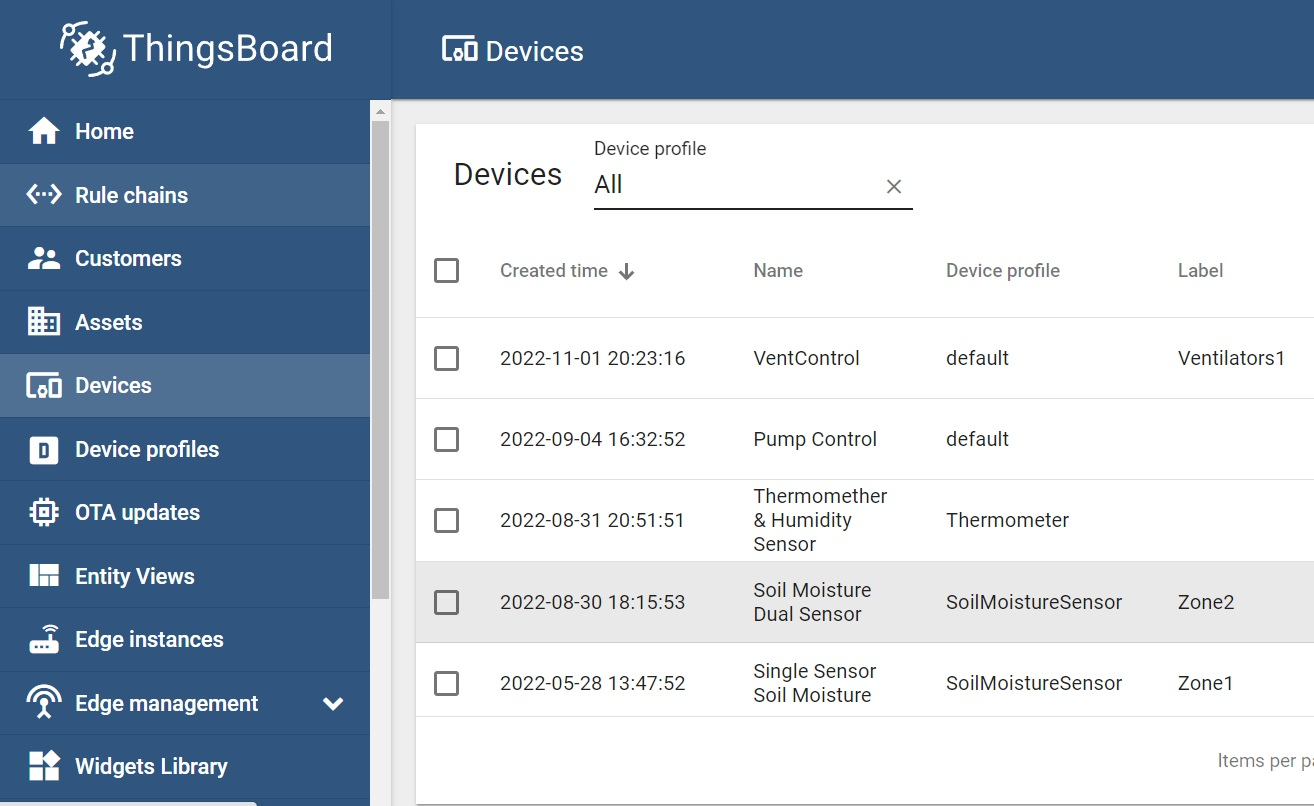
\includegraphics[width=0.9\textwidth]{./Figures/chapter3/TB_Devices4.jpg}
	    \caption[Listado de dispositivos del proyecto]{Listado de dispositivos del proyecto.}
	    \label{fig:tb_devices3}
     \end{subfigure}
     \hfill
     \begin{subfigure}[b]{0.75\textwidth}
	     \centering
	     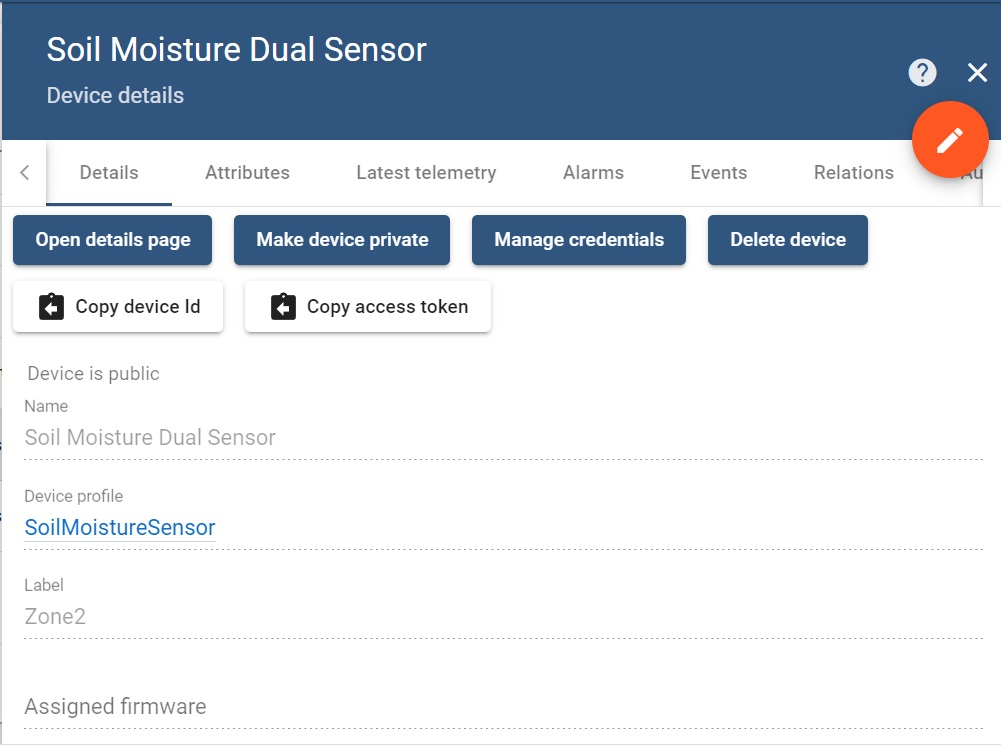
\includegraphics[width=0.9\textwidth]{./Figures/chapter3/TB_Devices5.jpg}
	     \caption[Configuración de las características de un sensor]{Configuración de las características de un sensor.}
	    \label{fig:tb_devices4}
     \end{subfigure}
    \caption[Pantallas de manejo de dispositivos creados en el proyecto]{Pantallas de manejo de dispositivos creados en el proyecto.}
	\label{fig:tb_devices}	
\end{figure}



\subsection{Reglas de automatización}
\label{sec:Reglas de automatización}
 
 
ThingsBoard posee un motor de reglas \citep{TB_Rules} para la creación de flujos de trabajo basados en eventos. Una de sus principales ventajas es la de permitir el desarrollo de automatizaciones bajo la metodología \textit{low-code/no-code} \citep{lcnc}.

Las reglas se componen principalmente de:
 
 \begin{itemize}
 \item Mensaje: cualquier evento que ingrese, por ejemplo datos provenientes de un dispositivo, un pedido a través de la API REST (HTTP) o un requerimiento RPC.
 \item Nodo de regla: función para el filtrado, transformación o acción que se ejecuta sobre un mensaje entrante y que puede producir mensajes salientes.
% \item Cadena: los nodos se conectan entre sí por medio de relaciones de forma tal que la salida de un nodo es enviada a los próximos nodos conectados.
\item Conexión de nodo de regla: los nodos pueden vincularse entre sí mediante relaciones, de manera que la salida de uno es enviada a los próximos nodos conectados. Cada relación tiene una etiqueta que identifica su significado lógico, generalmente del tipo ``éxito'' o ``fracaso''.
\item Cadena de reglas: grupo lógico de nodos de reglas y sus conexiones.

 \end{itemize}


El procesamiento de mensajes ofrece tres resultados posibles: éxito, error y \textit{timeout} (tiempo excedido).  Se obtiene un resultado exitoso cuando el último nodo de regla en la cadena completa correctamente el procesamiento. Se obtiene error cuando en el nodo se produce un fallo al operar sobre un mensaje y no existe un mecanismo para manejarlo. Por último, se establece un \textit{timeout} cuando el tiempo total de procesamiento supera el umbral configurado.



Para el proyecto se desarrollaron una o más reglas por subsistema, de manera de conectar a las unidades de control con los respectivos sensores que informan sobre el estado del invernadero y para el manejo de alertas a los usuarios. La figura \ref{fig:rule_riego} muestra, a manera de ejemplo, un fragmento de la regla creada para el control de riego a partir de los mensajes recibidos desde los sensores de humedad del suelo. Allí se visualizan los nodos en diferentes colores de acuerdo a su función y las cadenas como las flechas que los unen.

\begin{figure}[!h]
	\centering
	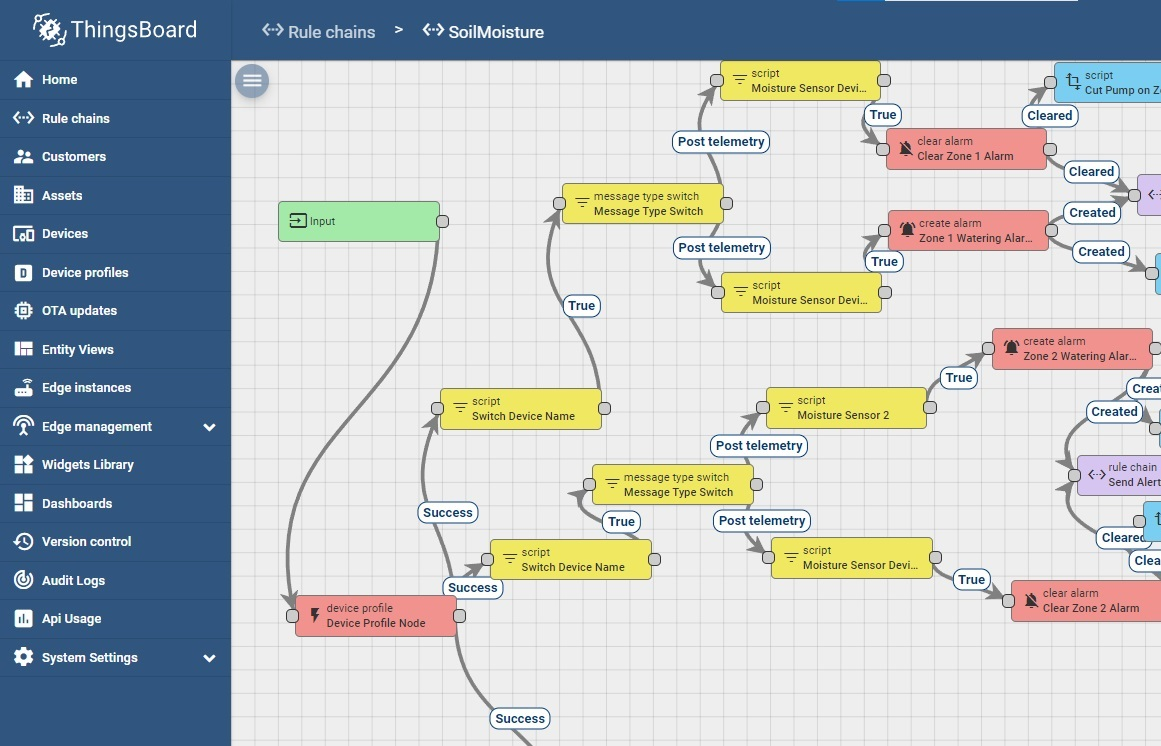
\includegraphics[width=1\textwidth]{./Figures/chapter3/TB_Rule_Soil 2.jpg}
	\caption[Fragmento de regla de automatización para el control de riego]{Fragmento de regla de automatización para el control de riego.}
	\label{fig:rule_riego}
\end{figure}

\subsection{Interfaz de manejo remoto}
\label{sec:Interfaz de manejo remoto}

%Para el acceso de usuarios a consultar el o manejar el invernadero desde Internet se evaluaron dos opciones:
%\begin{itemize}
%\item ngrok \citep{ngrok} es un servicio que ofrece publicar de forma segura una aplicación no expuesta a Internet. Dado que para el uso personal se requiere una suscripción anual y el pago de una licencia personal, el cliente descartó la solución.
%\item Telegram: mediante el servicio de \textit{bot} y la amplia disponibilidad de SDKs\
%\end{itemize}


Para permitir que los usuarios conozcan el estado del invernadero vía Internet, se desarrolló una aplicación en Python que se integra al \textit{bot} de Telegram mediante la librería SDK python-telegram-bot. Este programa fue alojado en la misma Raspberry Pi donde corre ThingsBoard.


Se trata de un bucle que contacta al \textit{bot} de Telegram periódicamente en busca de mensajes nuevos. Al detectar la llegada de alguno, el programa identifica si se corresponde con alguno de los comandos definidos y de ser así, envía una solicitud HTTP a la aplicación central. En base a la respuesta recibida, la interfaz confecciona un mensaje que es enviado al usuario por medio del \textit{bot}. La figura \ref{fig:telegram_status} muestra un ejemplo de mensaje de estado del invernadero.

Además, el servicio de \textit{bot} se utilizó para el envío de alertas a  usuarios. Para ello se crearon nodos en las reglas de automatización de la aplicación central que, ante ciertos eventos, disparan una solicitud HTTP POST al \textit{bot} con el mensaje de alerta como se ilustra en la figura \ref{fig:telegram_alerts}.

%\begin{subfigure}[!h]
%	\centering
%	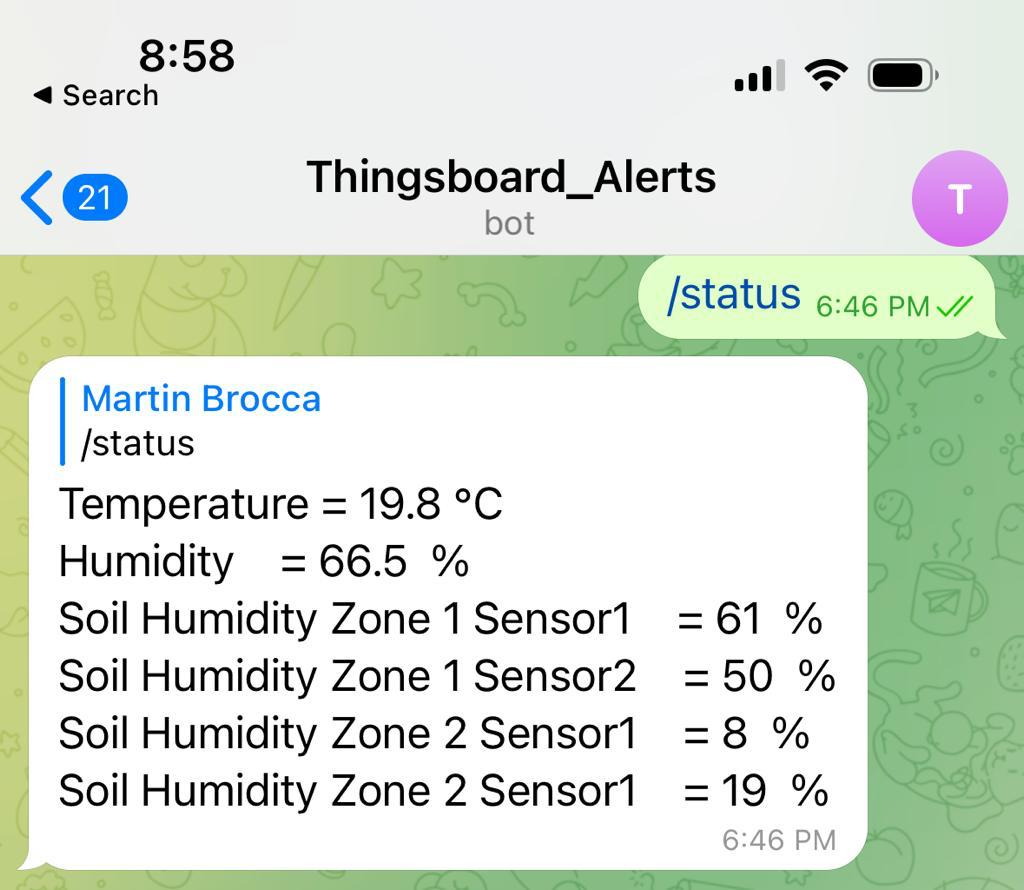
\includegraphics[width=0.5\textwidth]{./Figures/Telegram_Status.jpg}
%	\caption[Reporte de estado mediante el \textit{bot} de Telegram]{Reporte de estado mediante el \textit{bot} de Telegram.}
%	\label{fig:telegram_status}
%\end{subfigure}


\begin{figure}[!htpb]
     \centering
     \begin{subfigure}[b]{0.45\textwidth}
	    \centering
	    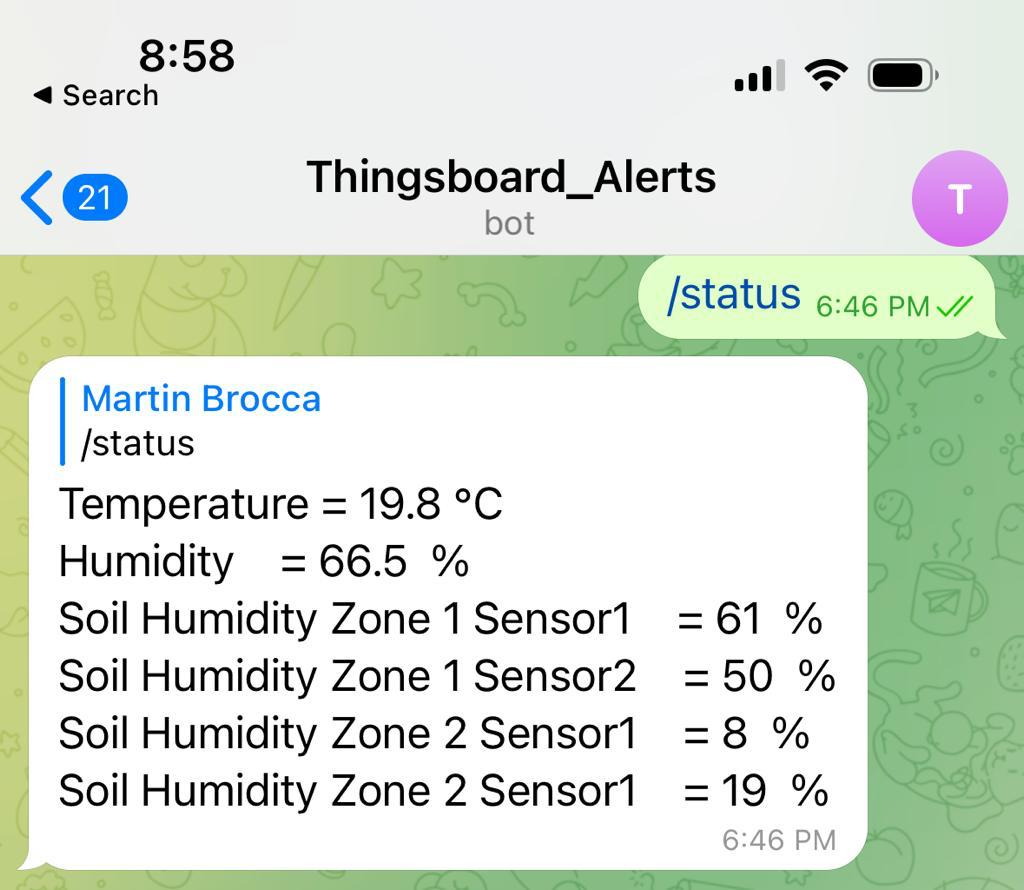
\includegraphics[width=0.9\textwidth]{./Figures/Telegram_Status.jpg}
	     \caption[Reporte de estado]{Reporte de estado.}
	     \label{fig:telegram_status}
     \end{subfigure}
     \hfill
     \begin{subfigure}[b]{0.45\textwidth}
	\centering
	    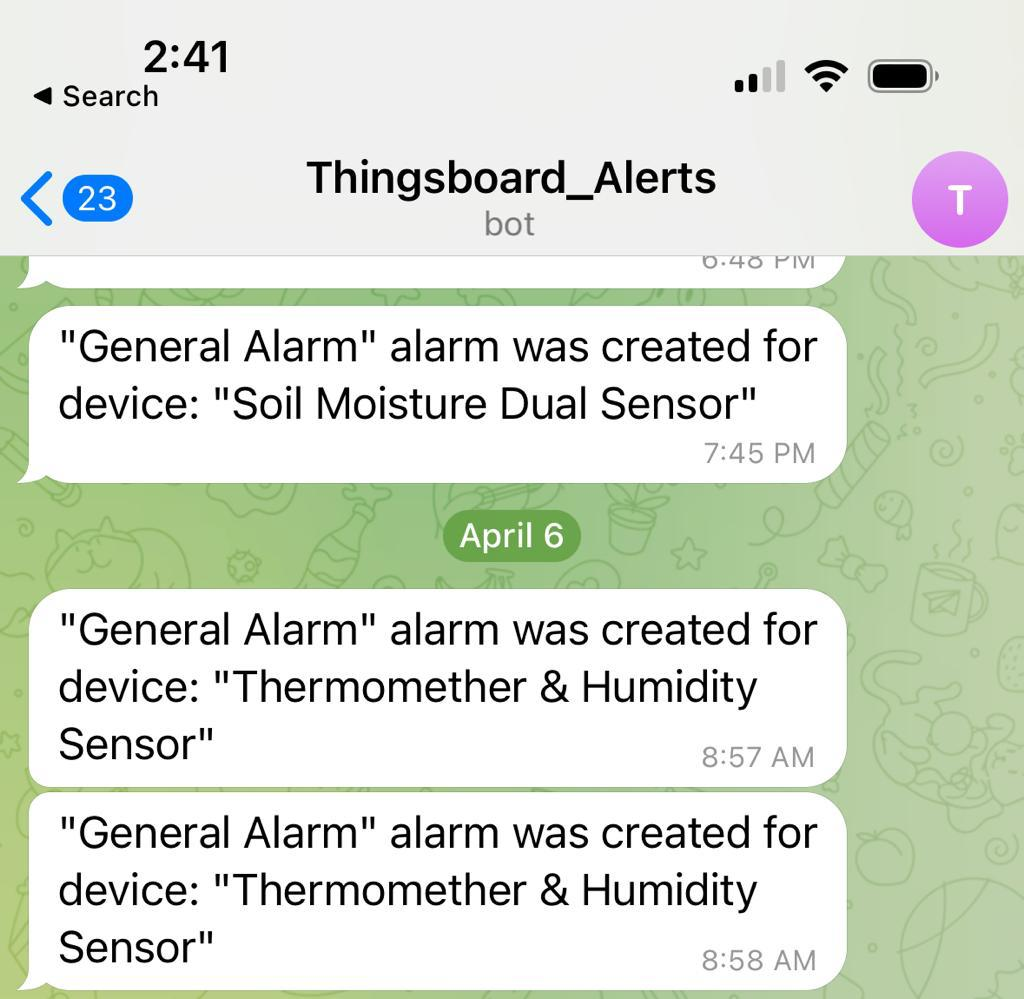
\includegraphics[width=0.9\textwidth]{./Figures/TB_Alert.jpg}
	     \caption[Mensaje de alerta en Telegram]{Mensaje de alerta en Telegram.}
	     \label{fig:telegram_alerts}
     \end{subfigure}	
	   \hfill
        \caption[Uso del \textit{bot} de Telegram ]{Uso del \textit{bot} de Telegram .}
        \label{fig:Telegram_bot}
\end{figure}





%\begin{figure}[!h]
%	\centering
%	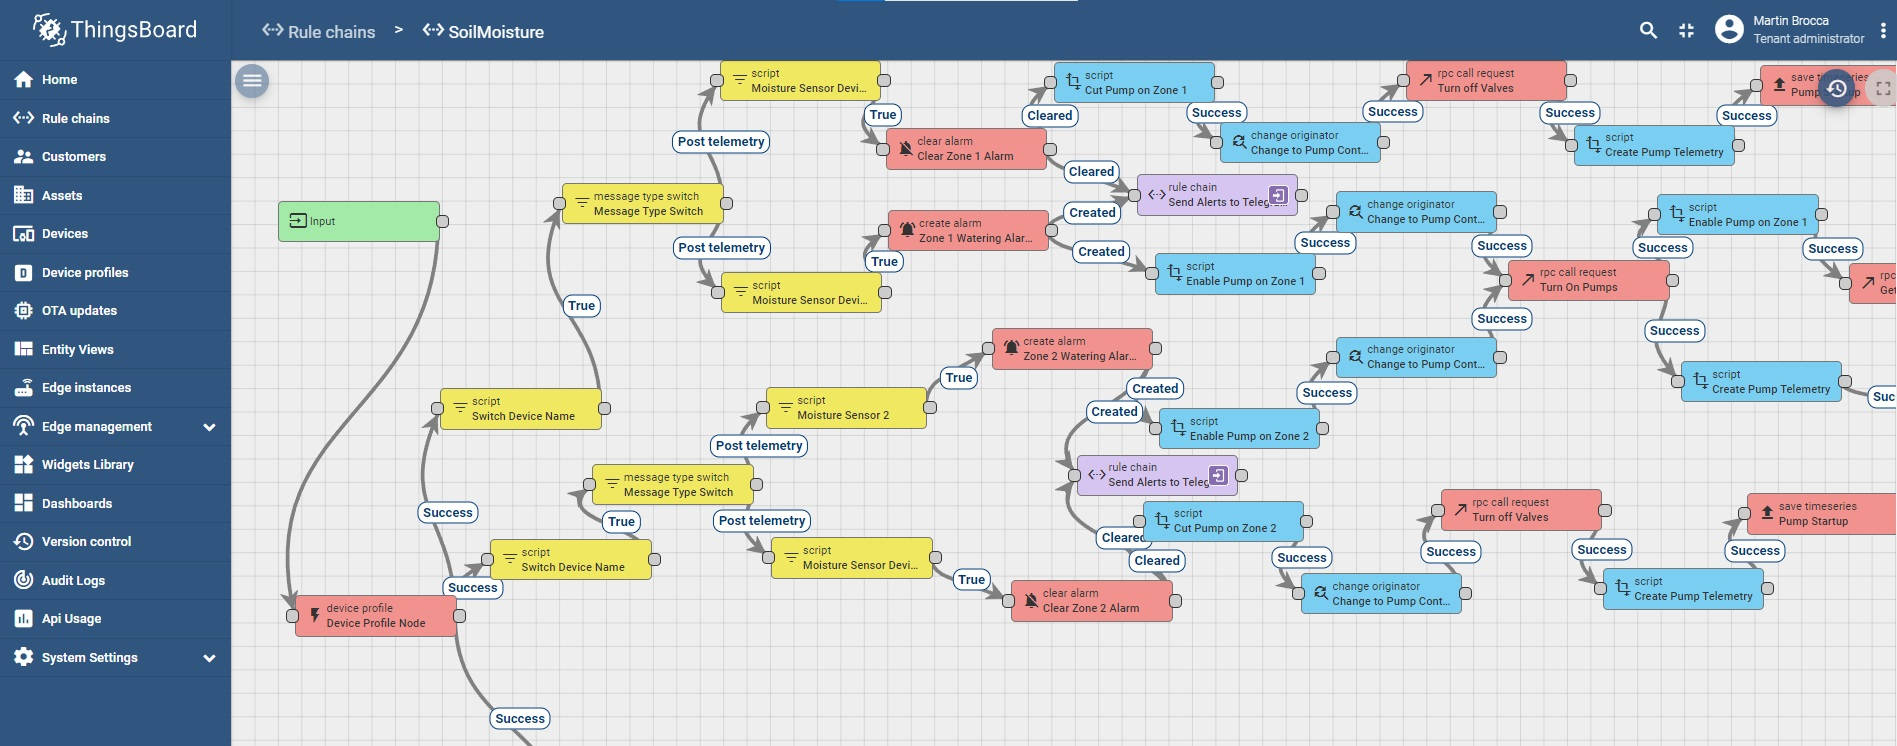
\includegraphics[width=0.9\textwidth]{./Figures/chapter3/TB_Rule_Soil.jpg}
%	\caption[Regla de automatización para el control de riego]{Regla de automatización para el control de riego.}
%	\label{fig:rule_riego}
%\end{figure}




\section{Ciberseguridad del sistema}
\label{sec:Ciberseguridad del sistema}



Por tratarse de un proyecto hogareño, el cliente no cuenta con la infraestructura de autenticación ni con una CA para proveer certificados a los dispositivos o a la aplicación central.
Por este motivo se decidió utilizar un certificado autofirmado para encriptar las comunicaciones entre los módulos y ThingsBoard. Sin embargo, el uso de este tipo de certificados tiene la desventaja de carecer del respaldo de una entidad que garantice su autenticidad, por lo que es necesario realizar configuraciones explícitas para forzar la confianza.


Durante el proceso de desarrollo se siguieron las buenas prácticas para el manejo de contraseñas y tokens de autenticación, evitando divulgar estos valores en los repositorios públicos.




